\chapter{Validation croisée entre les simulateurs}
Ce chapitre présente une comparaison des simulateurs selon les paramètres des simulation critiques: courant dans les électroaimants, tension aux bornes des électroaimants, courant à l'entrée de l'AFE, tension du bus CC, courants et tensions dans les IGBT. Les sous-modèles se séparent en plusieurs catégories, soit les simulations représentant l'AFE, ceux représentant le convertisseur CC-CC et ceux représentant un montage avec un AFE et un convertisseur CC-CC. Il est à noté que le temps de simulation qui est employé pour fins d'analyse est de 1$\mu$s. 

\section{Comparaison entre PSIM et SPS}
Cette section décrit des comparaisons faites sur le fonctionnement des éléments de bases fondamentaux pour le projet, dans les simulateurs PSIM et SPS.
\subsection{Algorithmes de simulation sur PSIM et SPS}
PSIM et SPS utilisent des méthodes de résolution différentes. SPS est un outil de simulation puissant et générique. Il établit un système d'équations d'états à partir du modèle de simulation; ces équations permettant de déterminer la solution du circuit. Les éléments non-linéaires sont modélisés comme des sources de courant. Les interrupteurs sont modélisés par une faible résistance en conduction et une forte résistance en blocage. Afin d'obtenir des modèles discrets, SPS discrétise les équations d'états continues en utilisant la méthode de Tustin  \footnote{http://www.mathworks.com/products/simpower/description4.html, 17 avril 2014}, la figure \ref{fig_solving_SPS} présente un résumé schématique de l'implémentation. Afin d'augmenter la vitesse de simulation de l'électronique de puissance, SPS utilise un algorithme dans lequel les commutations sont idéales. Il existe deux méthodes de détection des passages par 0 dans SPS, soit la méthode Tustin (équivalente à une méthode trapézoïdale) et la méthode Backward Euler. La méthode trapézoïdale offre une meilleur précision pour un temps de calcul fixe, mais peut parfois présenter des oscillations numériques. La méthode Backward Euler est moins précise pour un pas de simulation donné, mais permet d'éviter les oscillations numériques. PSIM implémente les modèles au moyen d'une matrice d'admittance nodale\footnote{http://powersimtech.com/support/frequently-asked-questions/, 17 avril 2014}. Les interrupteurs sont idéaux et représentés par une résistance faible en conduction et par une résistance élevée en blocage. La méthode de simulation de PSIM est moins adaptée à l'étude des transitoires pour l'électronique. Elle est cependant plus rapide et permet des études de plus haut niveau. La méthode de détection des passages par 0 de PSIM est une méthode trapézoïdale. 

\begin{figure}
\makebox[\textwidth][c]{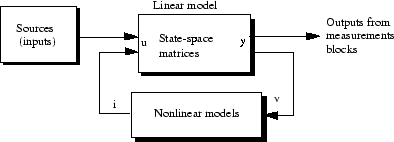
\includegraphics[scale=0.7]{Fig/Comp/improving_performance5.png}}
\caption{Méthode de solution des systèmes implantée dans SPS}
\label{fig_solving_SPS}
\end{figure}

\subsection{Comparaison des modèles d'IGBT}

\begin{figure}[htb]
\makebox[\textwidth][c]{\includegraphics[scale=0.5]{fig/Comp/IGBT.jpg}}
\caption{Commutation d'un IGBT à un pas de calcul de 5$\mu$s}.
\label{IG}
\end{figure}

Les IGBT sont les interrupteurs utilisés dans chacun des sous-modèles simulés du projet. On remarque sur la figure \ref{IG} que le  courant traversant l'IGBT est identique dans le cas d'un IGBT sur une charge résistive de 50k$\Omega$. Le pas de calcul employé sur les deux plateformes est de 5$\mu$s. L'indice de modulation des IGBT est de 0.5 et la fréquence de commutation de 1kKHz. Le montage est alimenté par une tension continue de 1kV et possède une résistance interne de 0.01$\Omega$. 

Sur SPS, l'IGBT possède un snubber RC intégré, tandis que sur PSIM il faut l'incorporer manuellement. Pour les deux simulations, le snubber employé est une résistance de 100k$\Omega$.
 
\subsection{Contrôleur proportionnel-intégrateur (PI)}
L'implantation des blocs PI est différente entre SPS et PSIM. Sur SPS, il est possible d'obtenir une forme idéale ainsi qu'une forme parallèle, tandis que sur PSIM, les blocs par défaut ne comportent que la forme idéale. La forme parallèle doit être implantée manuellement. On remarque sur la figure \ref{PI} que les résultats sont identiques entre une implantation manuelle sur PSIM et le bloc par défaut de SPS. La valeur du gain intégrateur du PI est de 50 et celle du gain proportionnel de 0.071. 

\begin{figure}[htb]
\makebox[\textwidth][c]{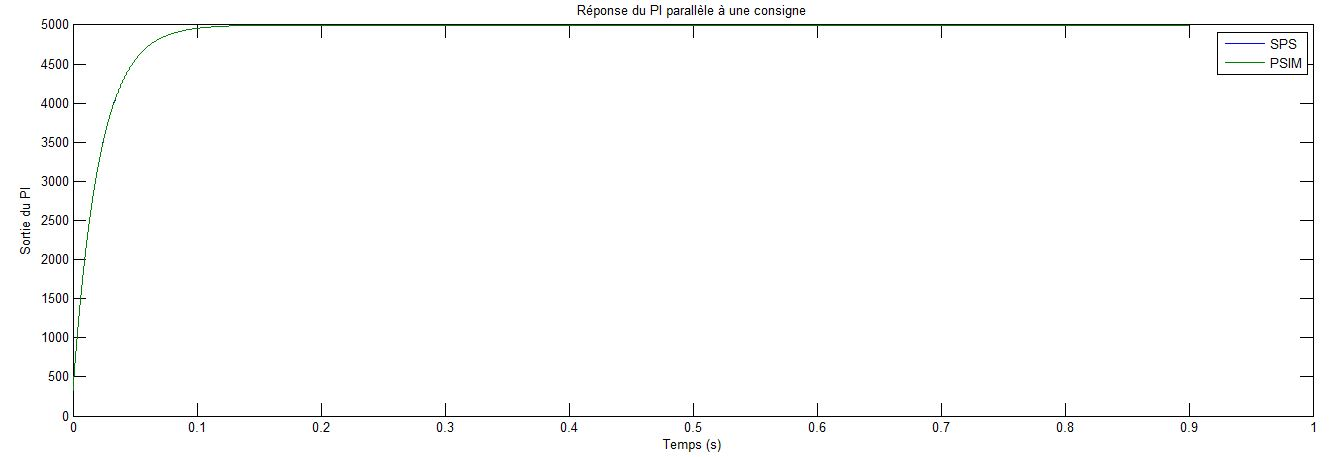
\includegraphics[scale=0.5]{fig/Comp/PI.jpg}}
\caption{Réponse d'un contrôleur PI suite à une consigne d'erreur}.
\label{PI}
\end{figure}

\clearpage
\subsection{Calibration des contrôleurs (PI)}
Les contrôleurs PI sont calibrés en utilisant des modèles continus équivalents des charges alimentées par les convertisseurs et ce, en excluant l'impact de la modulation. L'objectif étant d'obtenir la constante de temps dominante du circuit. Soit un circuit RL série, qui représente les électroaimants à alimenter, il est possible d'établir que la constante de temps dominante du contrôleur PI du convertisseur est de $T_i = \tau = L/R$. Le modèle de base d'un contrôleur PI pouvant être représenté par une équation dans le domaine de Laplace de la forme: $H(s) = \frac{1 + K_p T_is}{T_i s}$. Il suffit par la suite de procéder à une analyse dynamique du comportement du convertisseur afin de déterminer le gain $K_p$ fournissant la réponse optimale. Suivant cela, il est nécessaire de procéder à une discrétisation du régulateur selon le pas de calcul, selon la méthode de Tustin. 
\section{Convertisseur CC-CC 4 quadrants à 4 interrupteurs IGBT}
Le hacheur 4 quadrants, à proprement parlé, est constitué de 4 interrupteurs IGBT commandés au moyen d'une régulation MLI. La figure \ref{i_hach} présente le circuit électrique associé à un tel convertisseur. Ce type de montage est un montage de base utilisé afin de valider le concept de fonctionnement d'un convertisseur CC-CC et d'établir la méthodologie de comparaison des simulations. Le tableau \ref{p_hash} présente les paramètres utilisés pour le hacheur 4 quadrants.

\begin{figure}[htb]
\makebox[\textwidth][c]{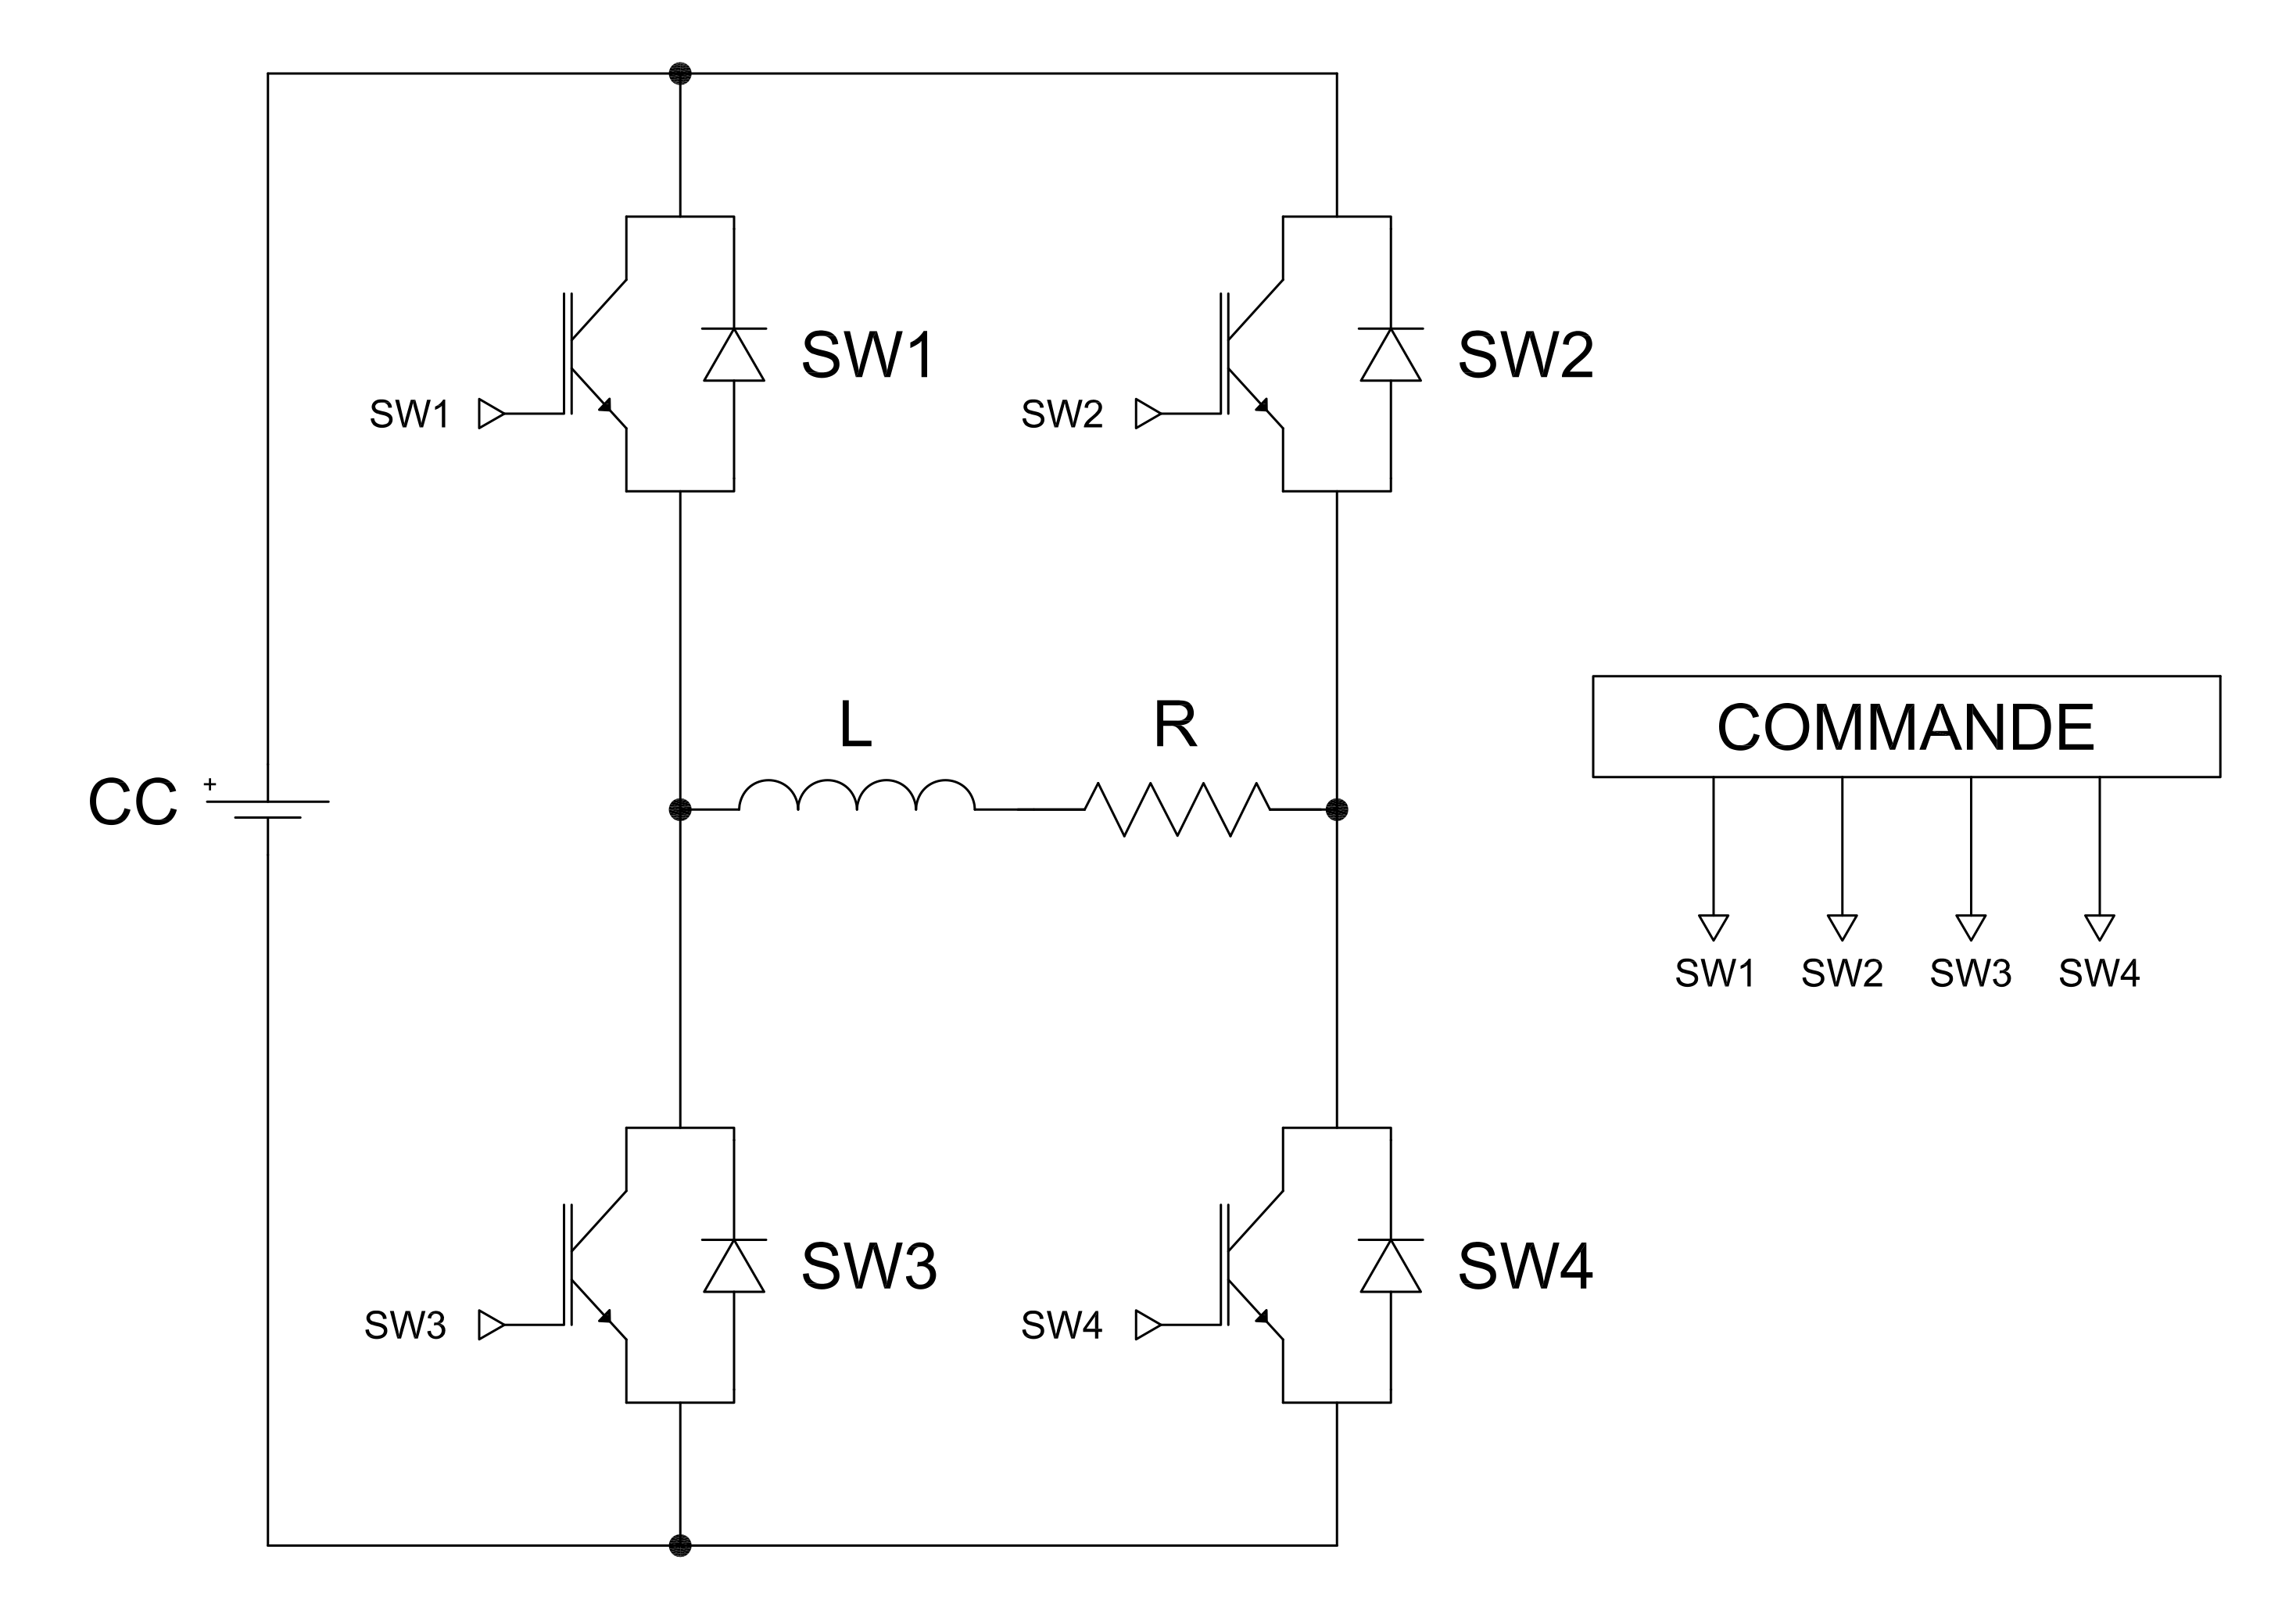
\includegraphics[scale=0.5]{fig/H4Q.png}}
\caption{Circuit électrique du convertisseur CC-CC 4 quadrants à 4 interrupteurs IGBT}
\label{i_hach}
\end{figure}

\begin{table}[htb]
\centering
\begin{tabular}{|l|c|} 
  \hline
  \textbf{Paramètre} & \textbf{Valeur}  \\
  \hline\hline
  Tension CC & 5000 V\\ \hline
  Fréquence de modulation & 1000 Hz\\ \hline
  Rapport cyclique maximal & 0.95 \\ \hline \hline
  \multicolumn{2}{|l|}{\textbf{IGBT}}\\ \hline
  Résistance interne & 0.001 $\Omega$\\
  Résistance du snubber & 100k $\Omega$\\ \hline \hline
   \multicolumn{2}{|l|}{\textbf{PI}}\\ \hline
  Gain proportionnel & 0.071 \\
  Gain intégrateur & 50 \\ \hline \hline
  \multicolumn{2}{|l|}{\textbf{Charge}}\\ \hline
  Résistance & 0.28 $\Omega$\\
  Inductance & 0.1 H\\
  \hline
\end{tabular}
\caption{Paramètres de simulation pour le convertisseur CC-CC à 4 interrupteurs}
\label{p_hash}
\end{table}

\subsection{Résultats de simulation pour SPS et PSIM pour un pas de calcul de 1$\mu$s}
Cette section présente les résultats de simulations du convertisseur CC-CC 4 quadrants, formé avec 4 interrupteurs IGBT, pour un pas de calcul de 1$\mu$s. 


\begin{figure}[htb]
\makebox[\textwidth][c]{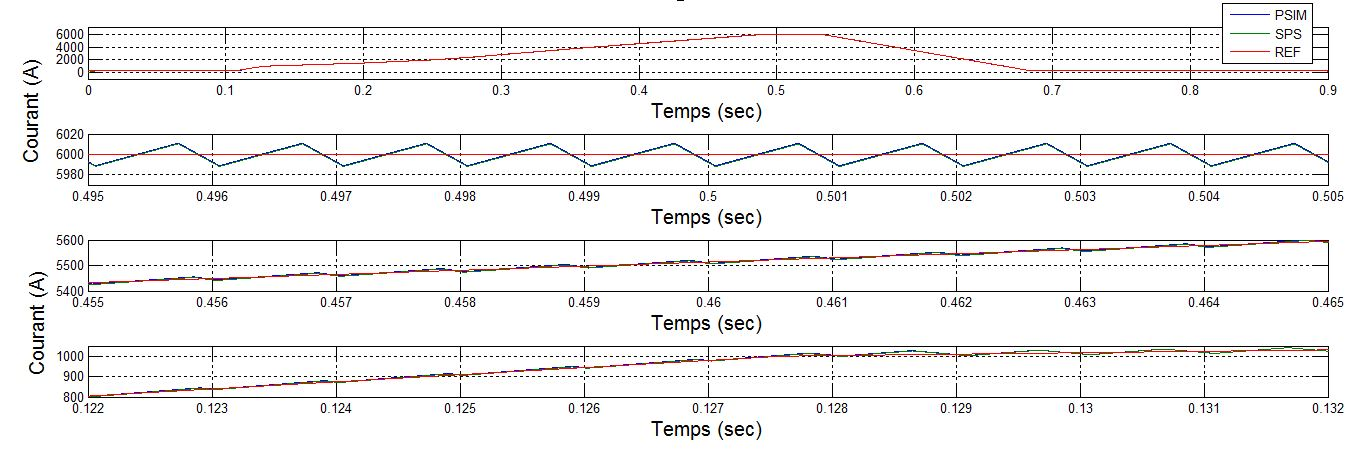
\includegraphics[scale=0.5]{fig/Hacheur4Quadrants/HacheurCourantCharge1u.jpg}}
\caption{Courant traversant la charge sur PSIM et SPS pour un pas de calcul de 1$\mu$s, pour le hacheur 4 quadrants}
\label{hc_cou_ch_1}
\end{figure}


\begin{figure}[htb]
\makebox[\textwidth][c]{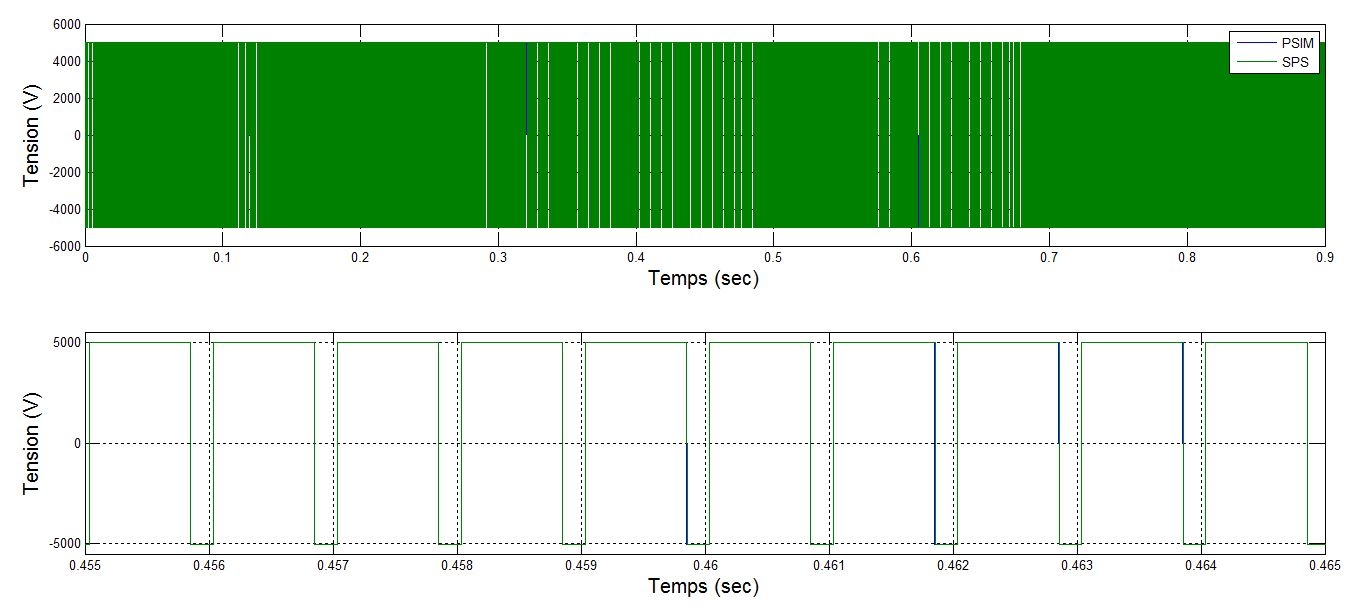
\includegraphics[scale=0.5]{fig/Hacheur4Quadrants/HacheurTensionCharge1u.jpg}}
\caption{Tension aux bornes de la charge sur PSIM et SPS pour un pas de calcul de 1$\mu$s, pour le hacheur 4 quadrants}
\label{hc_ten_ch_1}
\end{figure}


\begin{figure}[htb]
\makebox[\textwidth][c]{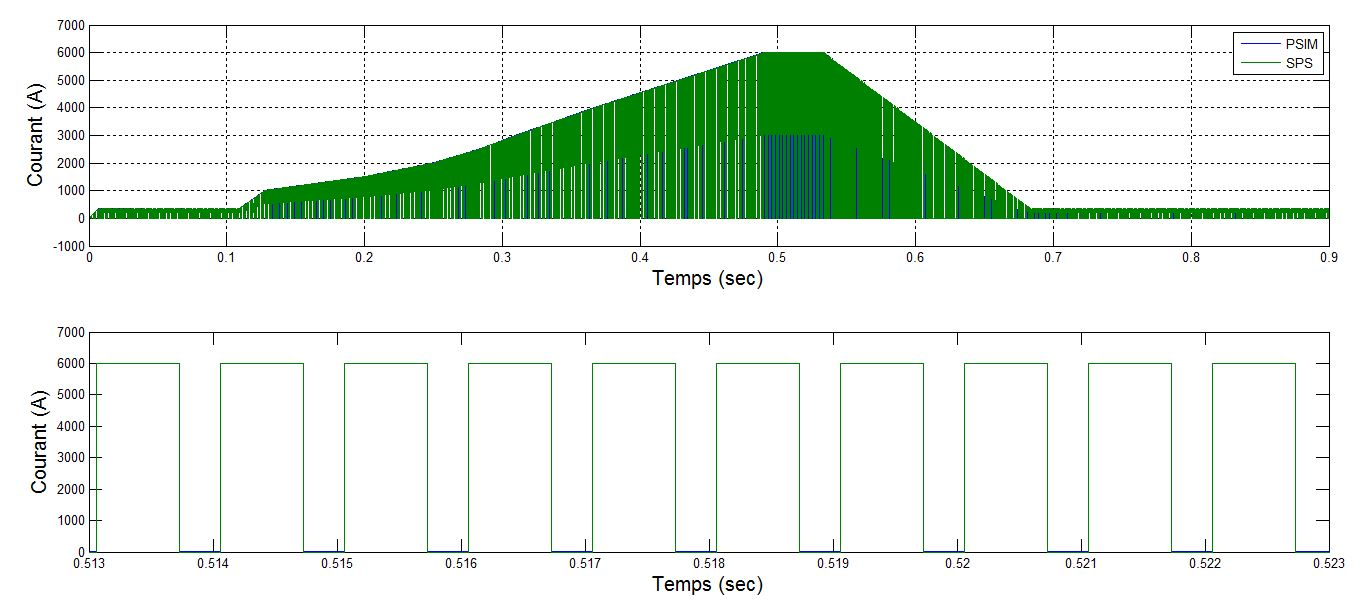
\includegraphics[scale=0.5]{fig/Hacheur4Quadrants/HacheurCourantIGBT1u.jpg}}
\caption{Courant traversant un IGBT sur PSIM et SPS pour un pas de calcul de 1$\mu$s, pour le hacheur 4 quadrants}
\label{hc_IG_cou_1}
\end{figure}

\begin{figure}[htb]
\makebox[\textwidth][c]{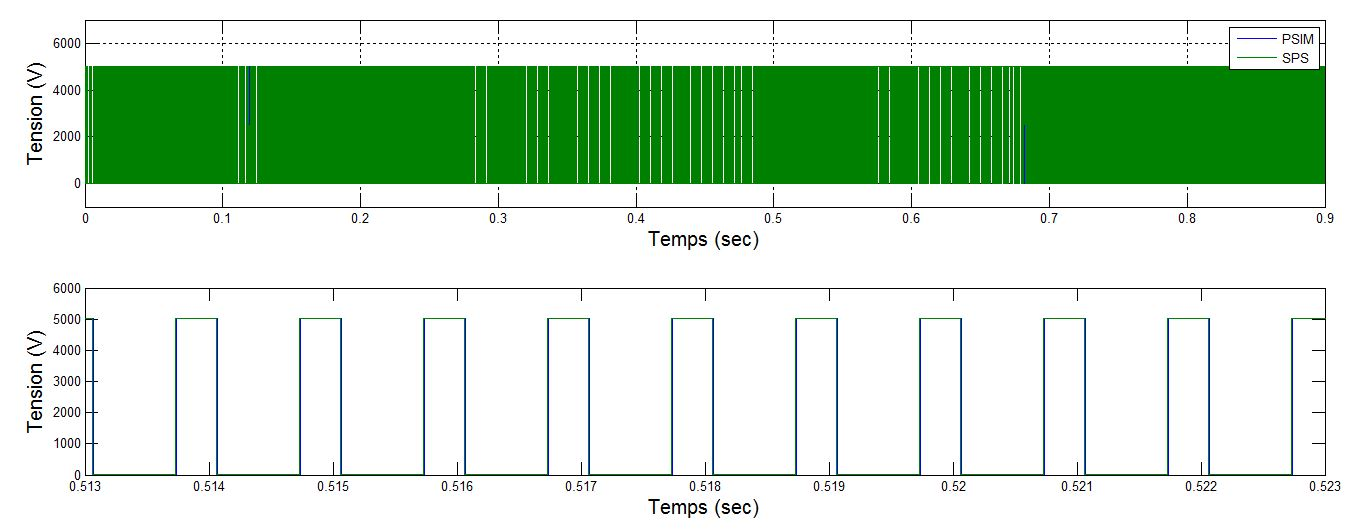
\includegraphics[scale=0.5]{fig/Hacheur4Quadrants/HacheurTensionIGBT1u.jpg}}
\caption{Tension aux bornes d'un IGBT sur PSIM et SPS pour un pas de calcul de 1$\mu$s, pour le hacheur 4 quadrants}
\label{hc_IG_ten_1}
\end{figure}


\clearpage
\subsection{Analyse des résultats comparatifs de SPS et de PSIM pour un pas de calcul de 1$\mu$s}

Les résultats obtenus pour la simulation du hacheur 4 quadrants permettent d'établir la méthodologie du projet. On note que les simulations confirment le fonctionnement dans la zone de maintien du courant à 6kA, ce qu'on peut remarquer à la figure \ref{hc_cou_ch_1}. Il est pratiquement impossible de discerner des différences dans les résultats de simulation, pour ce cas. À la même figure, il est possible de noter les courants dans les différentes phases du cycle des électroaimants. On remarque que les courbes de PSIM et SPS sont presque parfaitement superposées en montée. La figure \ref{hc_ten_ch_1} permet d'observer la tension aux bornes de la charge. On remarque qu'il est pratiquement impossible de discerner une différence à l'échelle de la commutation entre les simulations. La conclusion est identique pour les figures représentant la tension et le courant vus par l'un des IGBT. Cette simulation simple d'un convertisseur CC-CC permet d'asseoir la méthodologie de conception et d'observer le comportement du convertisseur CC-CC escompté Les considérations de filtrage de l'onde ont été prises en compte et on remarque qu'il ne semble pas y avoir une quantité de réammorçages excessives. La bande passante observée correspond donc à celle désirée et le comportement est corrélé à travers 2 simulateurs




\section{Convertisseur CC-CC 4 quadrants formé de 2 convertisseurs 3 niveaux NPC}
Le montage implanté au CERN est un convertisseur CC-CC formé de 2 onduleurs triphasés 3 niveaux NPC. La cellule supérieure est dénotée par DCP et la cellule inférieure par DCN. L'assemblage des onduleurs est tel qu'il permet le fonctionnement dans les 4 quadrants. Cette version reproduit le fonctionnement du hacheur 4 quadrants de base avec un plus grand degré de liberté. Il est composé au total de 24 interrupteurs IGBT/DIODE commandés par MLI ainsi que de 12 diodes de point milieu. La figure \ref{circuit_DCP_DCN} présente le circuit électrique du convertisseur. Le tableau \ref{p_DCP} présente les données utilisées pour ce sous-système.


\begin{figure}[htb]
\makebox[\textwidth][c]{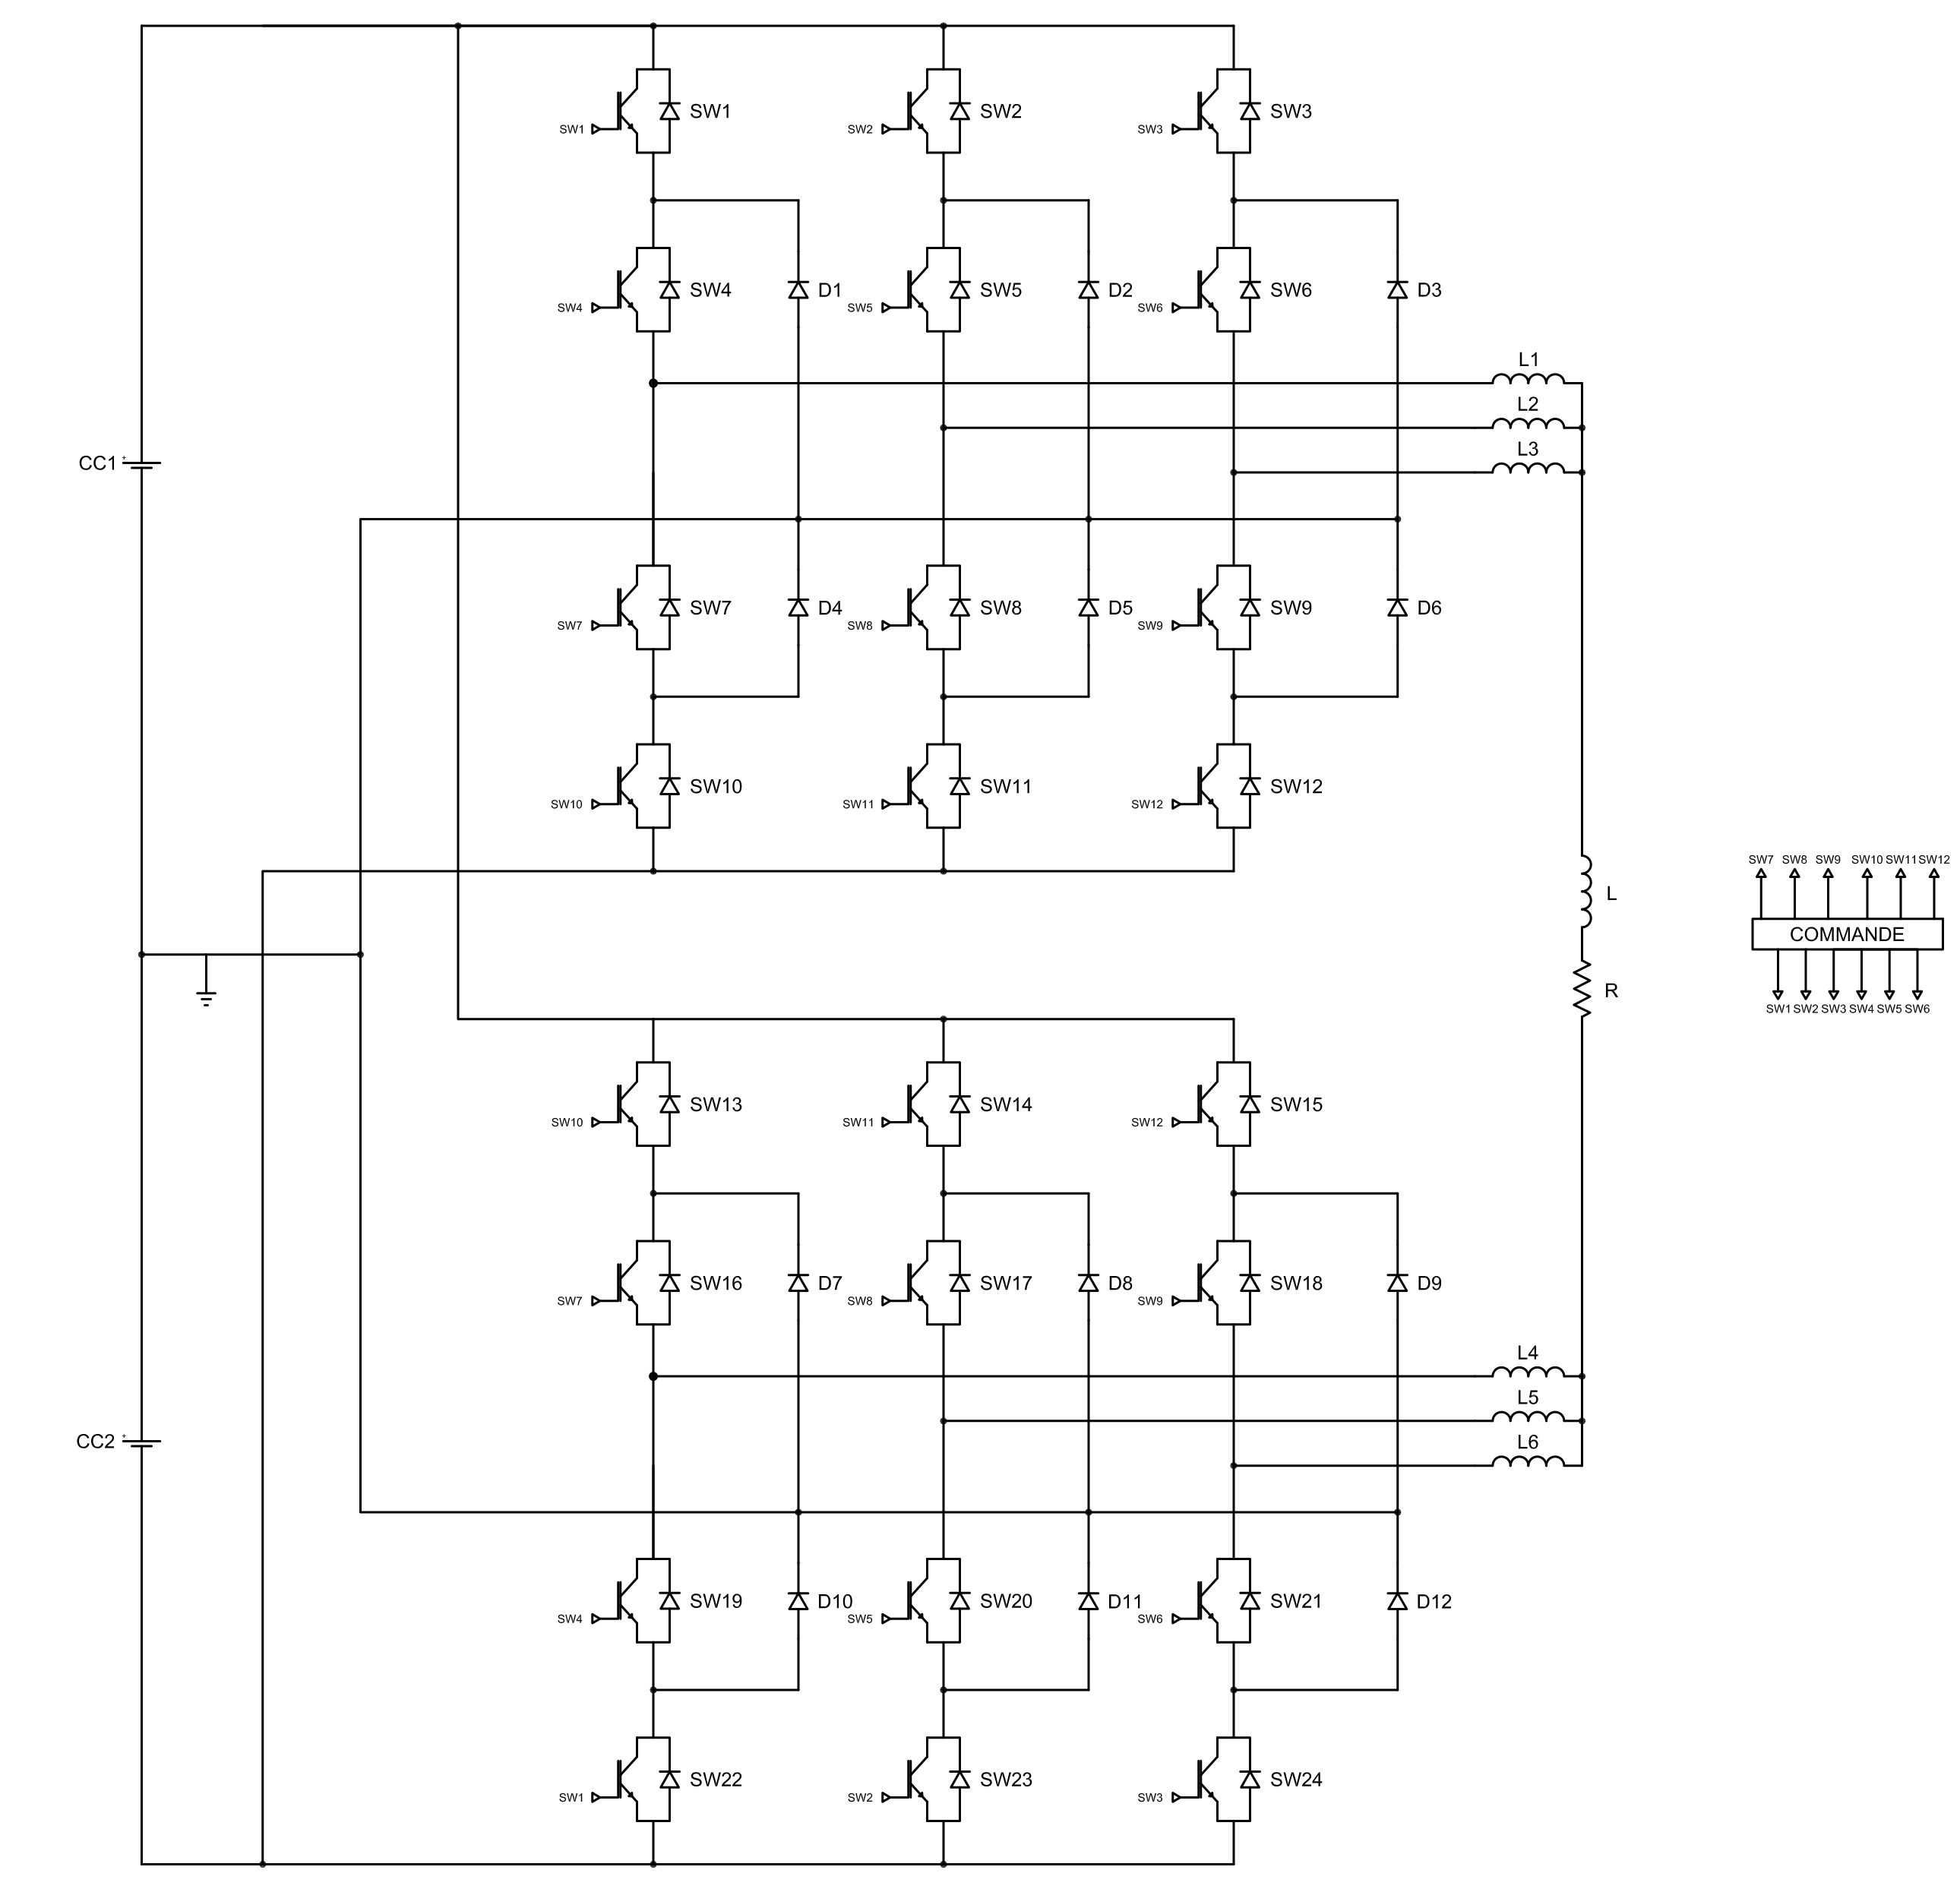
\includegraphics[scale=0.75]{fig/DCP_DCN.png}}
\caption{Circuit électrique du convertisseur CC-CC 4 quadrants formé de 2 convertisseurs 3 niveaux NPC}
\label{circuit_DCP_DCN}
\end{figure}


\begin{table}[htb]
\centering
\begin{tabular}{|l|c|} 
  \hline
  \textbf{Paramètre} & \textbf{Valeur}  \\
  \hline\hline
  Tension CC & 5000 V\\ \hline
  Fréquence de modulation & 1000 Hz\\ \hline
  Rapport cyclique maximal & 1 \\ \hline
  Inductance de couplage & 10e-6 H \\ \hline \hline
  \multicolumn{2}{|l|}{\textbf{IGBT}}\\ \hline
  Résistance interne & 0.001 $\Omega$\\
  Résistance du snubber  & 100k $\Omega$\\ \hline \hline
   \multicolumn{2}{|l|}{\textbf{PI}}\\ \hline
  Gain proportionnel & 1.5611 \\
  Gain intégrateur & 24.6 \\ \hline \hline
  \multicolumn{2}{|l|}{\textbf{Charge}}\\ \hline
  Résistance & 0.28 $\Omega$\\
  Inductance & 0.1 H \\
  \hline
\end{tabular}
\caption{Paramètres de simulation pour le DCP/DCN}
\label{p_DCP}
\end{table}
\clearpage


\subsection{Résultats de simulation pour SPS et PSIM pour un pas de calcul de 1$\mu$s}
Cette section présente les résultats de simulation obtenus sur PSIM et SPS pour le convertisseur CC-CC 4 quadrants formé de 2 cellules NPC 3 niveaux, pour un pas de calcul discret de 1$\mu$s.



\begin{figure}[htb]
\makebox[\textwidth][c]{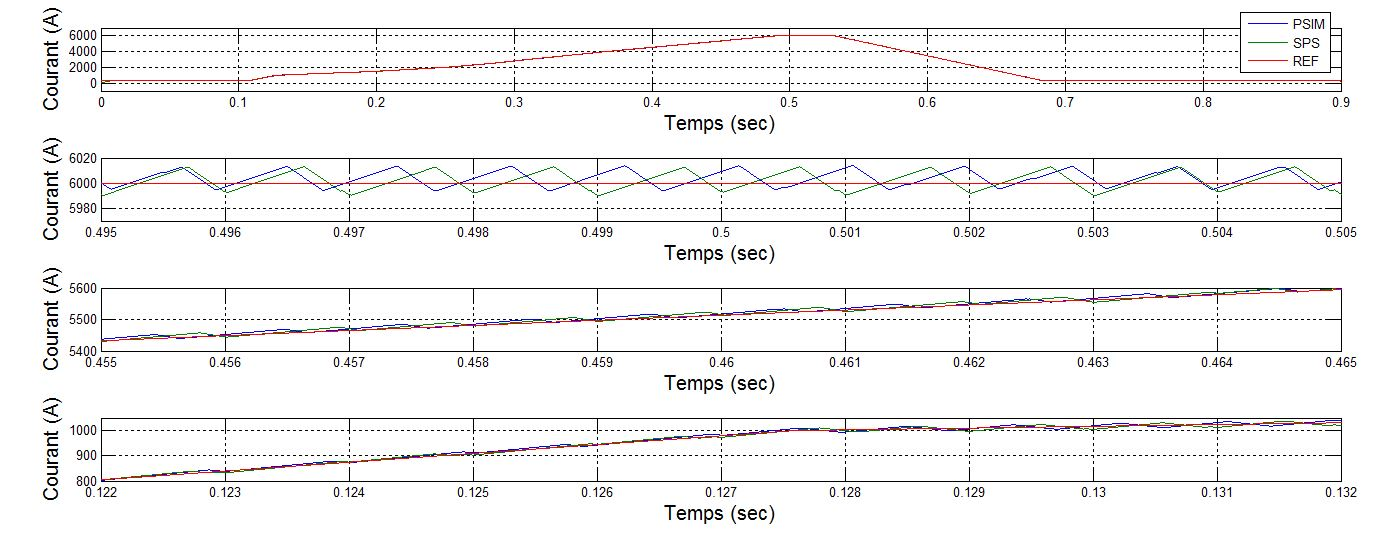
\includegraphics[scale=0.5]{fig/DCPDCN/DCPCourantCharge1u.jpg}}
\caption{Courant traversant la charge sur PSIM et SPS pour un pas de calcul de 1$\mu$s pour le DCP/DCN}
\label{DC_ch_cou_1}
\end{figure}



\begin{figure}[htb]
\makebox[\textwidth][c]{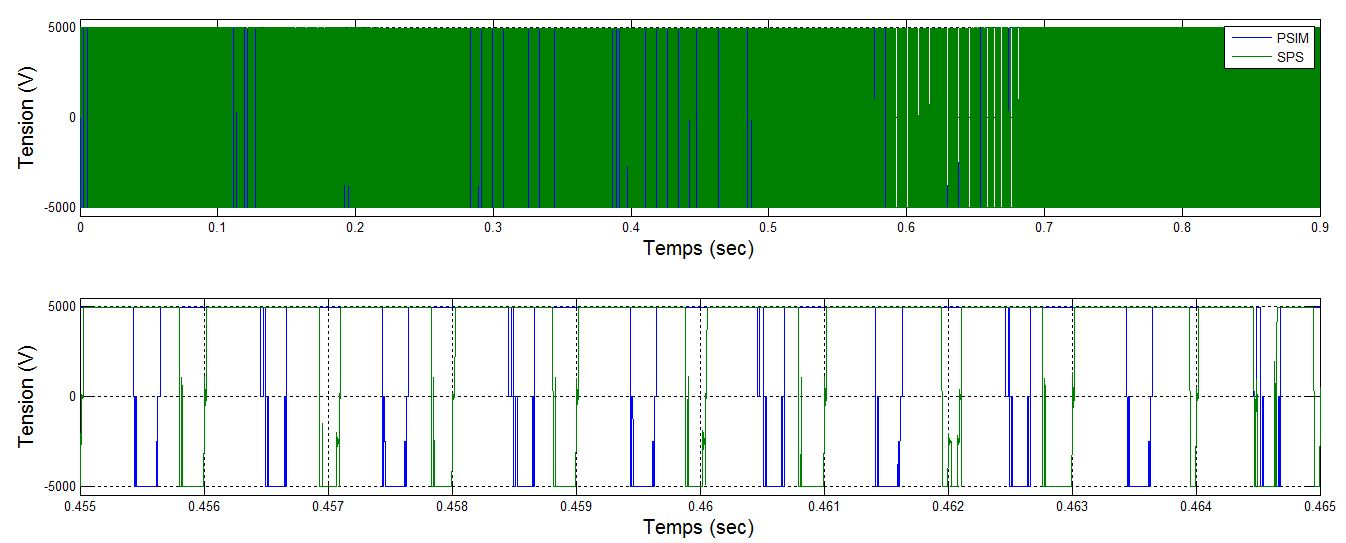
\includegraphics[scale=0.5]{fig/DCPDCN/DCPTensionCharge1u.jpg}}
\caption{Tension aux bornes de la charge sur PSIM et SPS pour un pas de calcul de 1$\mu$s pour le DCP/DCN}
\label{DC_ch_ten_1}
\end{figure}


\begin{figure}[htb]
\makebox[\textwidth][c]{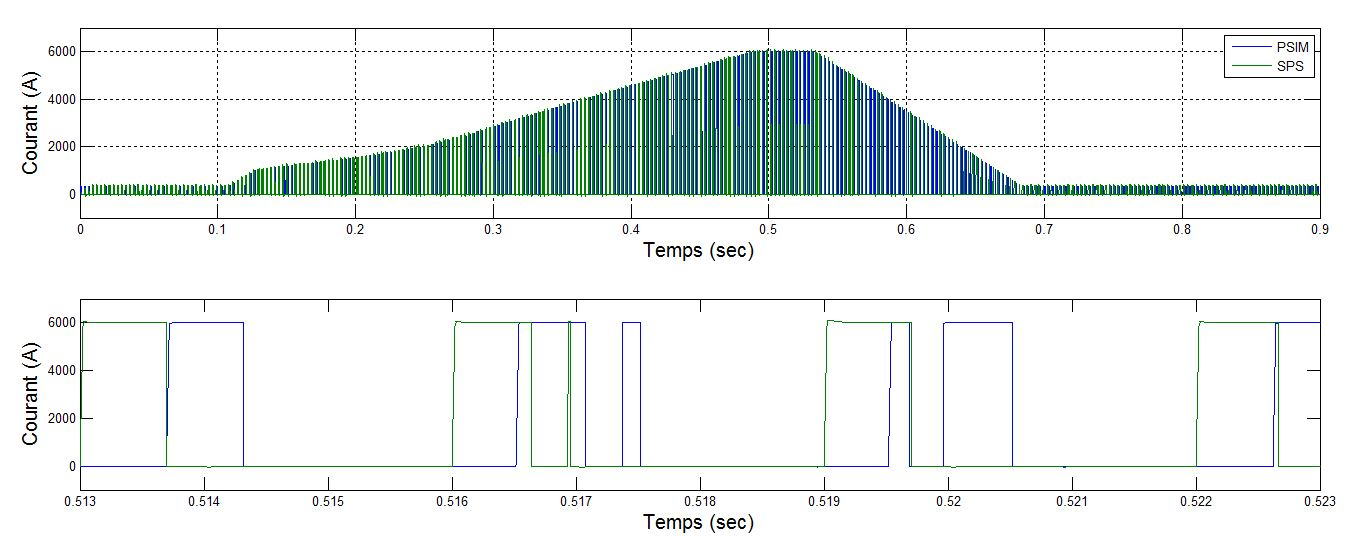
\includegraphics[scale=0.5]{fig/DCPDCN/DCPCourantIGBT1u.jpg}}
\caption{Courant traversant un IGBT sur PSIM et SPS pour un pas de calcul de 1$\mu$s pour le DCP/DCN}
\label{DC_IG_cou_1}
\end{figure}


\begin{figure}[htb]
\makebox[\textwidth][c]{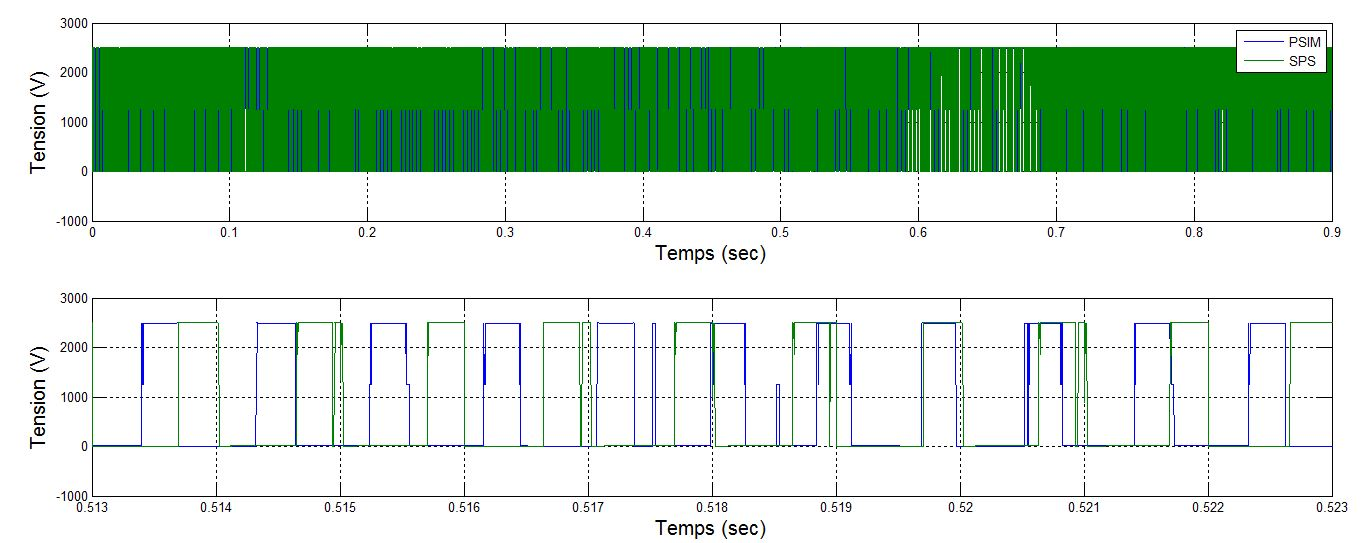
\includegraphics[scale=0.5]{fig/DCPDCN/DCPTensionIGBT1u.jpg}}
\caption{Tension aux bornes d'un IGBT sur PSIM et SPS pour un pas de calcul de 1$\mu$s pour le DCP/DCN}
\label{DC_IG_ten_1}
\end{figure}


\clearpage

\subsection{Analyse des résultats comparatifs de SPS et de PSIM pour un pas de calcul de 1$\mu$s}

La figure \ref{DC_ch_cou_1} présente le courant dans la charge de manière globale, dans la zone de maintien, en montée initiale et en montée rapide. On remarque dans la figure montrant le courant dans la charge dans la zone de maintien que la fréquence de l'un des 2 simulateurs glisse par rapport à l'autre. La simulation de PSIM utilisant une analyse nodale et SPS des matrices d'équations d'états, on se doute que la détection des passages par 0 ne s'effectue pas nécessairement de manière synchrone dans les 2 simulations. De plus, la discrétisation est effectuée de manière différente dans les 2 simulations, ce qui rend les instants de détection par 0 potentiellement différents dans les 2 simulations. Les paramètres de SPS ont été réglés de manière à utiliser une méthode similaire à une méthode trapézoïdale, mais qui n'est pas nécessairement implantée de la même façon. On comprend, par rapport au hacheur 4 quadrants simple, que l'augmentation de la taille de la matrice d'équations d'états (SPS) et l'augmentation de la matrice d'admittance nodale (PSIM) permettent de constater les différences cumulatives des 2 méthodes de résolution. Les formes de courant en montée initiale et rapide montrent le même phénomène qu'en maintien, soit un glissement de la fréquence. Cependant, il est à noter que la symétrie est préservée ainsi que les amplitudes des variations.
\section{AFE 2 niveaux avec contrôle par hystérésis débitant sur une source idéale}
L'AFE (Active Front End) est un redresseur triphasé permettant de réguler le facteur de puissance à l'entrée du montage. La charge étant une source idéale pour cette simulation, il est possible d'en observer le fonctionnement dans les 4 quadrants. Ce convertisseur CA/CC est constitué de 6 interrupteurs, soit 2 par bras. Ce système a pour fonction d'alimenter un bus CC et de maintenir sa tension à 5kV avec un facteur de puissance variable vu à l'entrée. Une méthode de contrôle par hystérésis est employée afin de réguler le courant (en amplitude et en phase) du côté du réseau. La figure \ref{circuit_AFE_IDEAL} présente le circuit électrique du convertisseur. Le tableau~\ref{p_AF_ID} présente les paramètres utilisés pour la simulation.

\begin{figure}[htb]
\makebox[\textwidth][c]{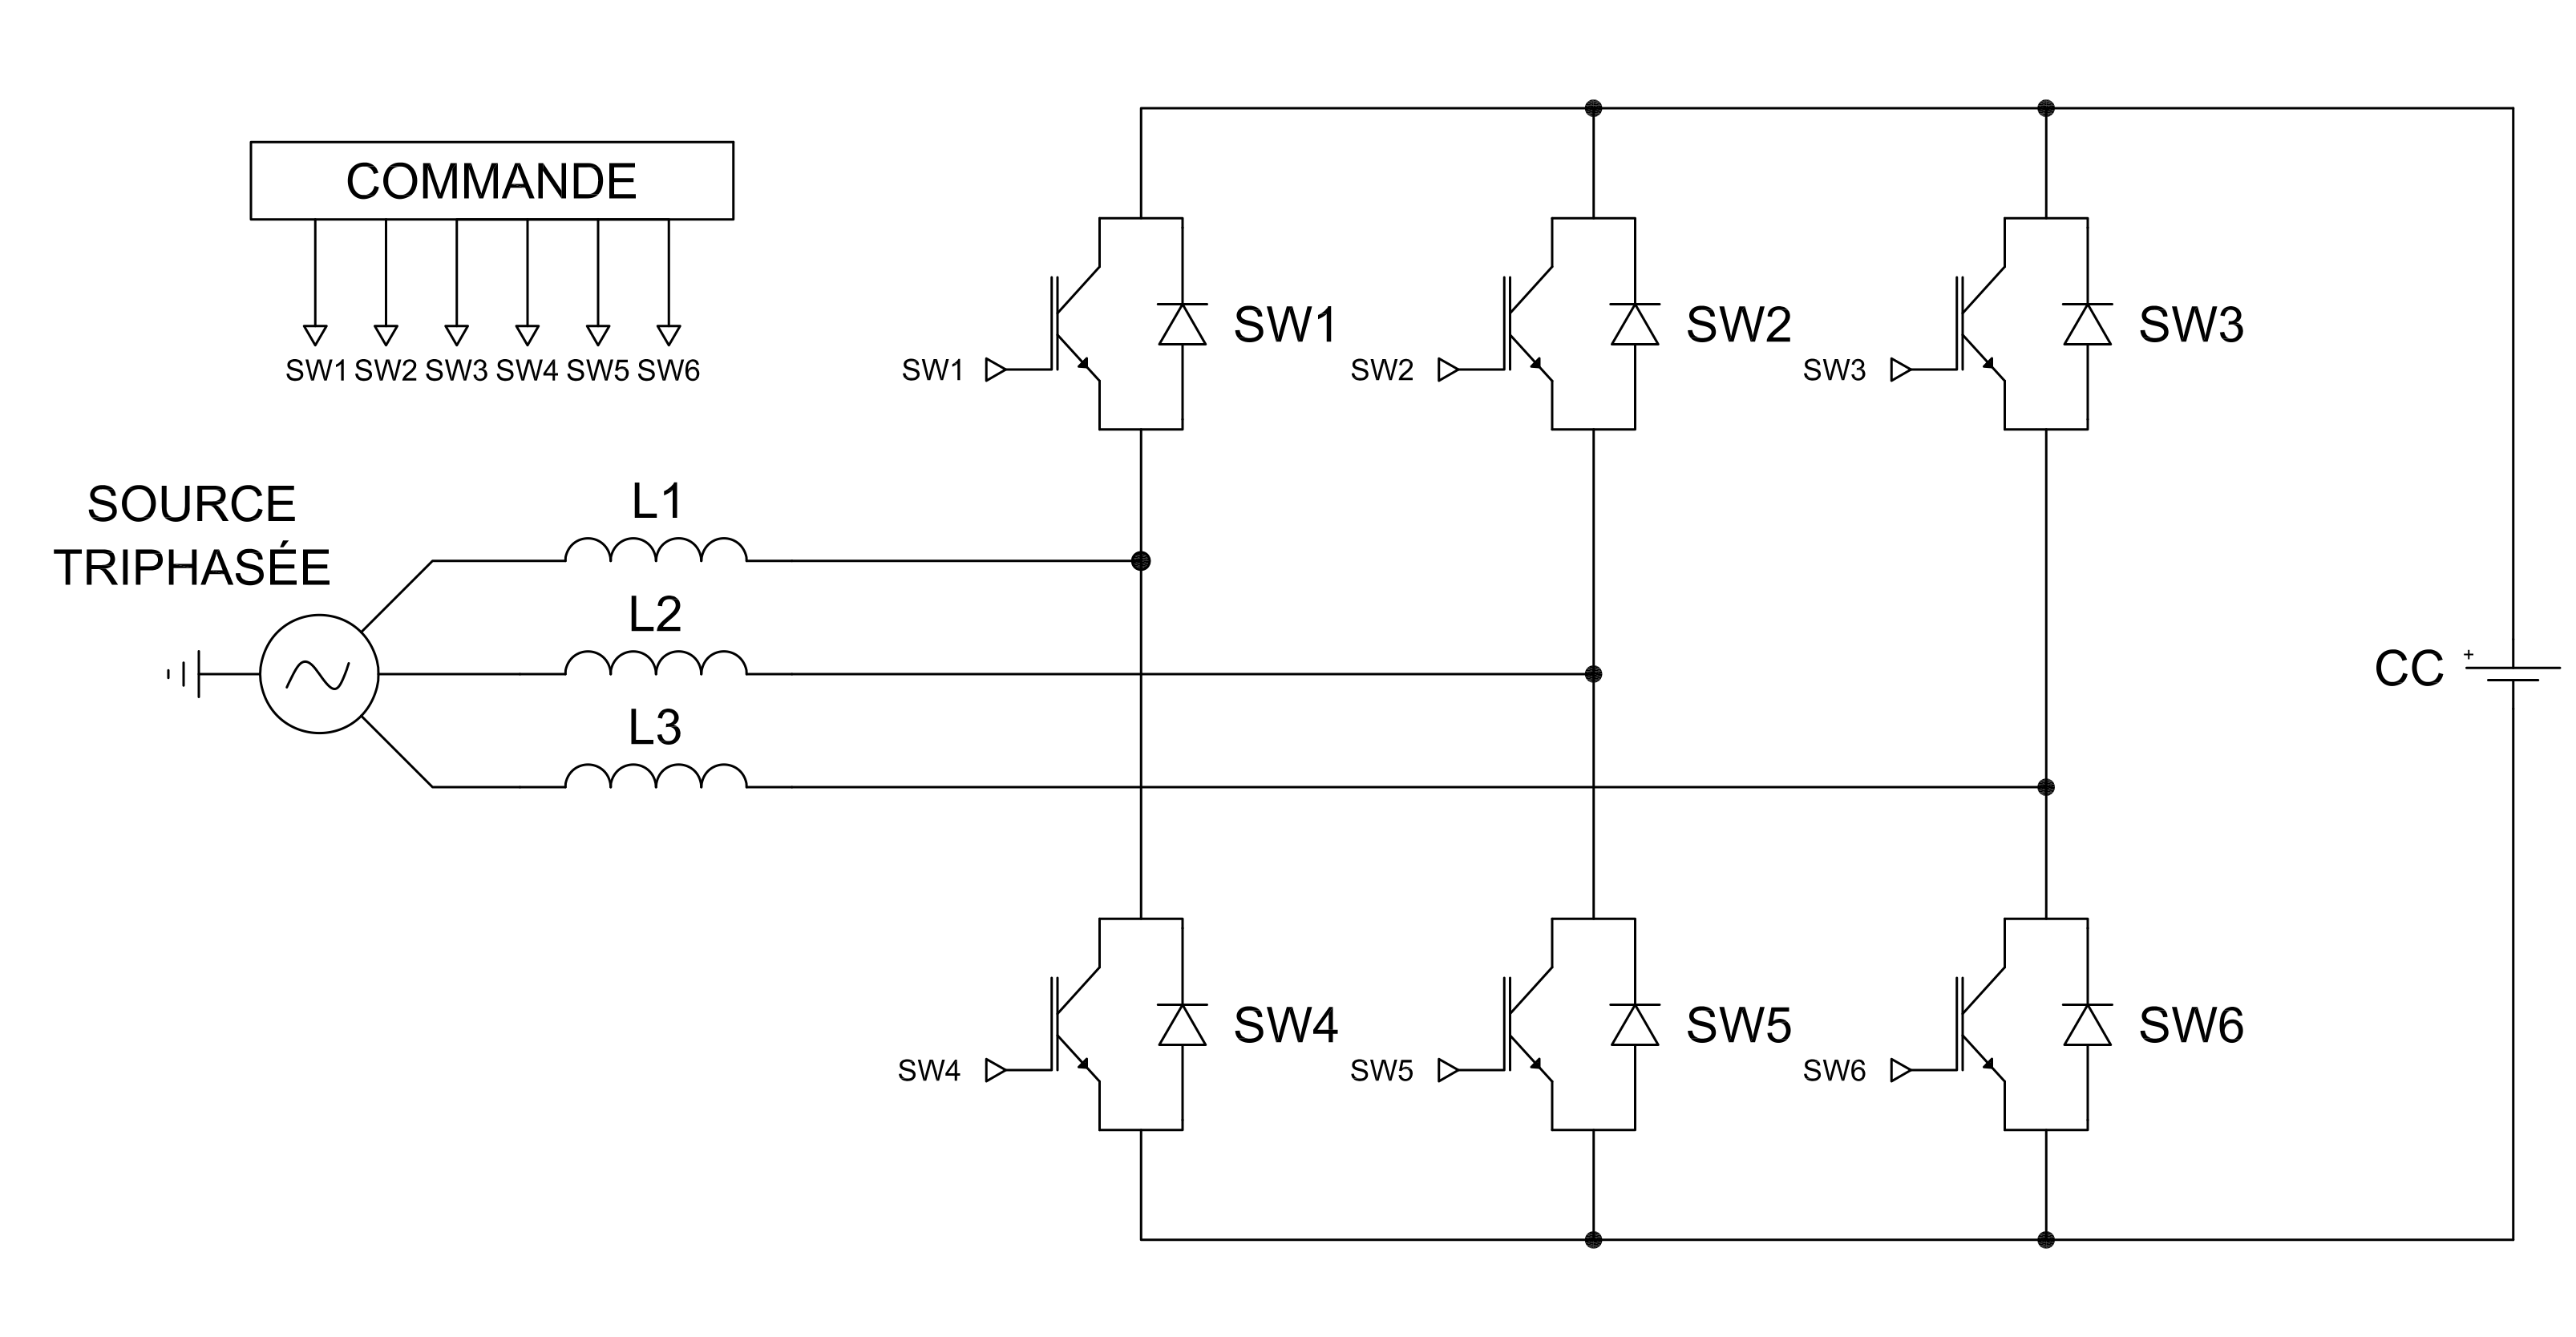
\includegraphics[scale=0.6]{fig/AFE_IDEAL.png}}
\caption{Circuit électrique de l'AFE 2 niveaux sur source parfaite}
\label{circuit_AFE_IDEAL}
\end{figure}


\begin{table}[htb]
\centering
\begin{tabular}{|l|c|} 
  \hline
  \textbf{Paramètre} & \textbf{Valeur}  \\
  \hline\hline
  Tension bus CC & 5000\\ \hline
  Courant référence & 1000A\\ \hline
  Seuil hystérésis & 450A\\ \hline
  Inductance côté AC& 81.487 mH\\ \hline
  Courant maximal à l'entrée& 1500A \\ \hline \hline
  \multicolumn{2}{|l|}{\textbf{IGBT}}\\ \hline
  Résistance interne & 0.001$\Omega$\\
  Résistance du snubber & 100k$\Omega$\\ \hline \hline
   \multicolumn{2}{|l|}{\textbf{PI de courant}}\\ \hline
  Gain proportionnel & 5 \\
  Gain intégrateur & 20 \\ \hline \hline
  \multicolumn{2}{|l|}{\textbf{PI de phase}}\\ \hline
  Gain proportionnel & 0.48 \\
  Gain intégrateur & 8 \\ \hline \hline
  \hline
\end{tabular}
\caption{Paramètres de simulation pour l'AFE débitant sur une source idéale}
\label{p_AF_ID}
\end{table}
\clearpage

\subsection{Résultats de simulation pour SPS et PSIM pour un pas de calcul de 1$\mu$s}
Cette section présente les résultats de simulation de l'AFE 2 niveaux avec contrôle par hystérésis, débitant sur une source idéale, pour un pas de calcul discret de 1$\mu$s. 


\begin{figure}[htb]
\makebox[\textwidth][c]{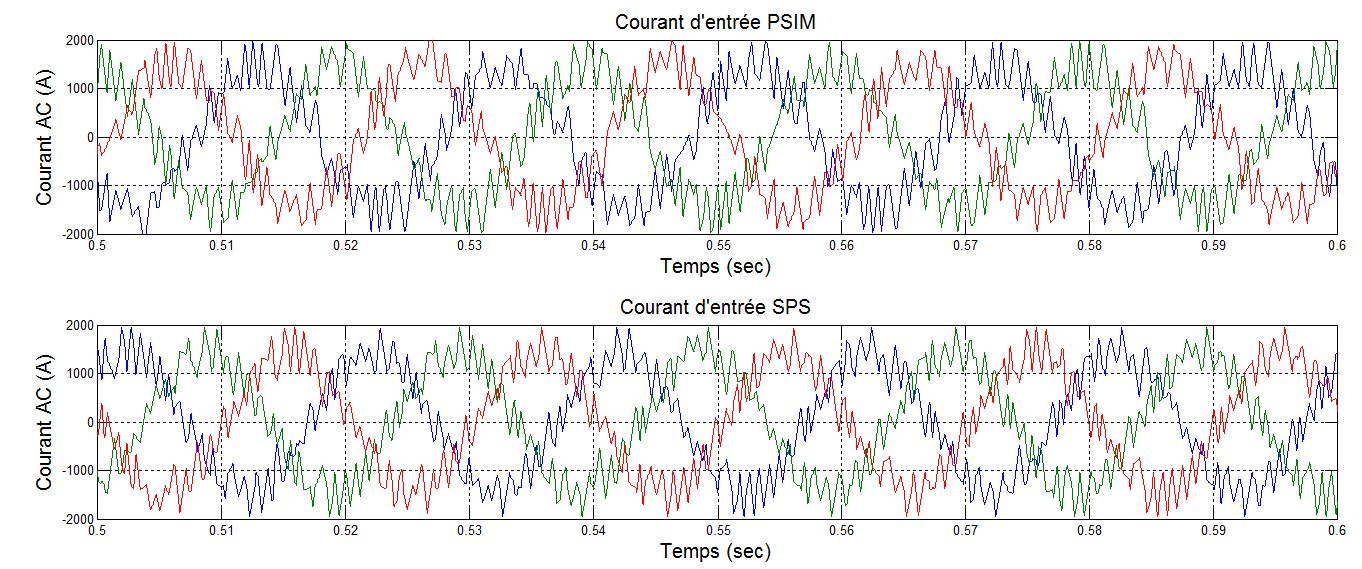
\includegraphics[scale=0.5]{fig/AFEIDEAL/CourantAC.jpg}}
\caption{Le courant d'entrée avec un pas de calcul de 1$\mu$s pour l'AFE 2 niveaux avec contrôle par hystérésis sur source idéale}
\label{AF_I_cou}
\end{figure}



\begin{figure}[htb]
\makebox[\textwidth][c]{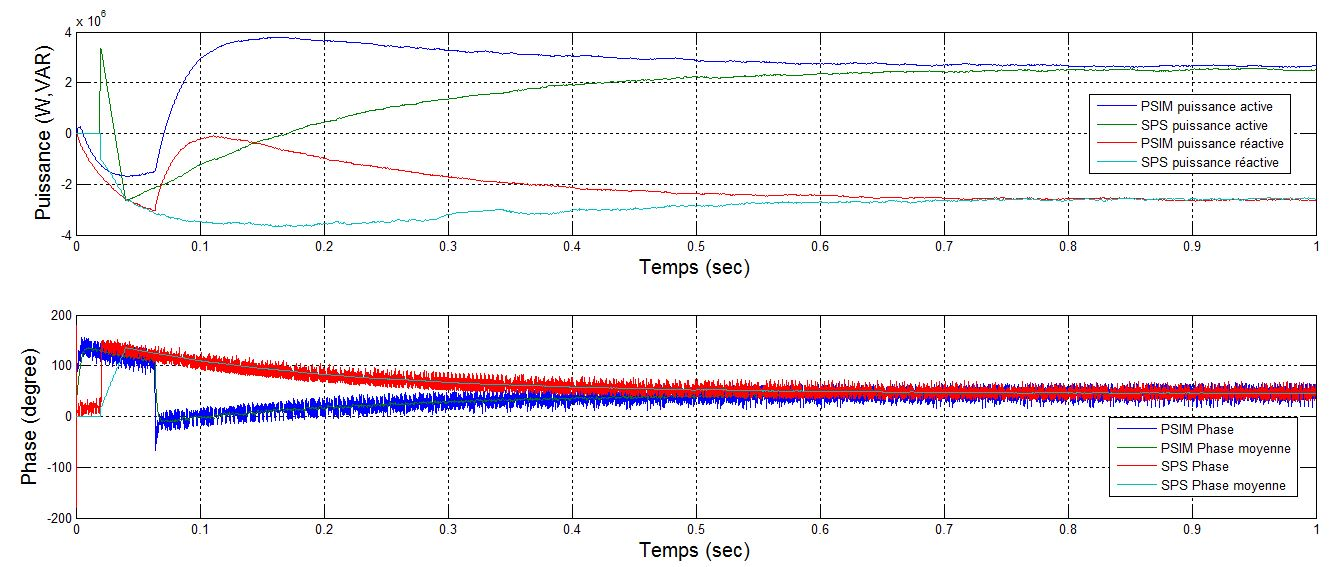
\includegraphics[scale=0.5]{fig/AFEIDEAL/pui45.jpg}}
\caption{Puissances active et réactive pour une courant déphasé de 45$^\circ$, pour un pas de calcul 1$\mu$s}
\label{AF_I_pui_45}
\end{figure}

\begin{figure}[htb]
\makebox[\textwidth][c]{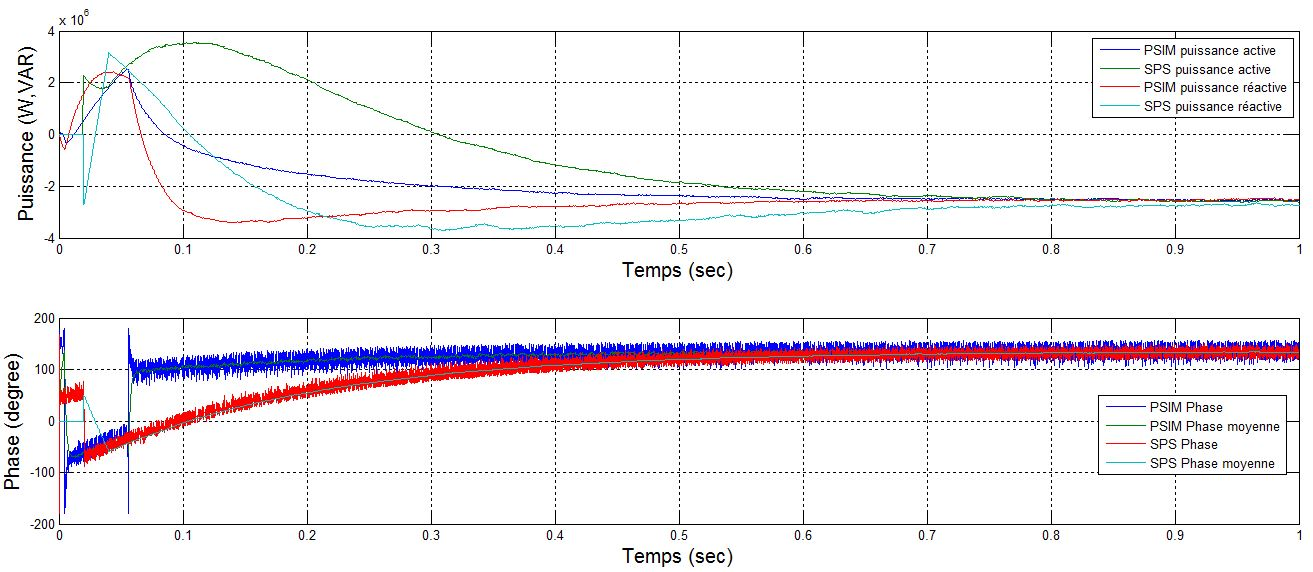
\includegraphics[scale=0.5]{fig/AFEIDEAL/pui135.jpg}}
\caption{Puissances active et réactive pour une courant déphasé de 135$^\circ$, pour un pas de calcul 1$\mu$s}
\label{AF_I_pui_135}
\end{figure}

\begin{figure}[htb]
\makebox[\textwidth][c]{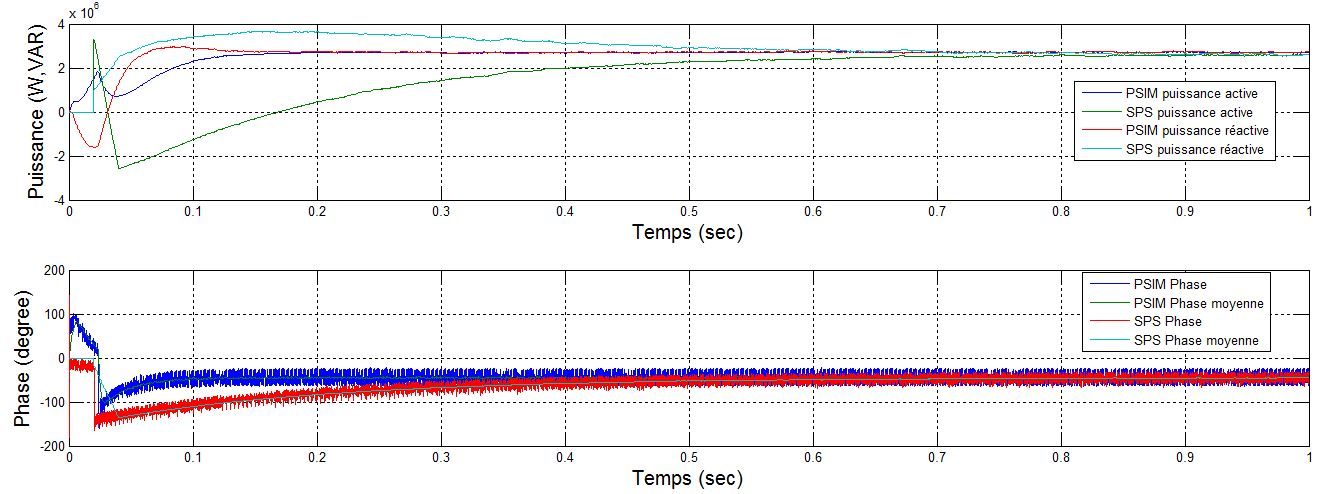
\includegraphics[scale=0.5]{fig/AFEIDEAL/pui_45.jpg}}
\caption{Puissances active et réactive pour une courant déphasé de -45$^\circ$, pour un pas de calcul 1$\mu$s}
\label{AF_I_pui__45}
\end{figure}

\begin{figure}[htb]
\makebox[\textwidth][c]{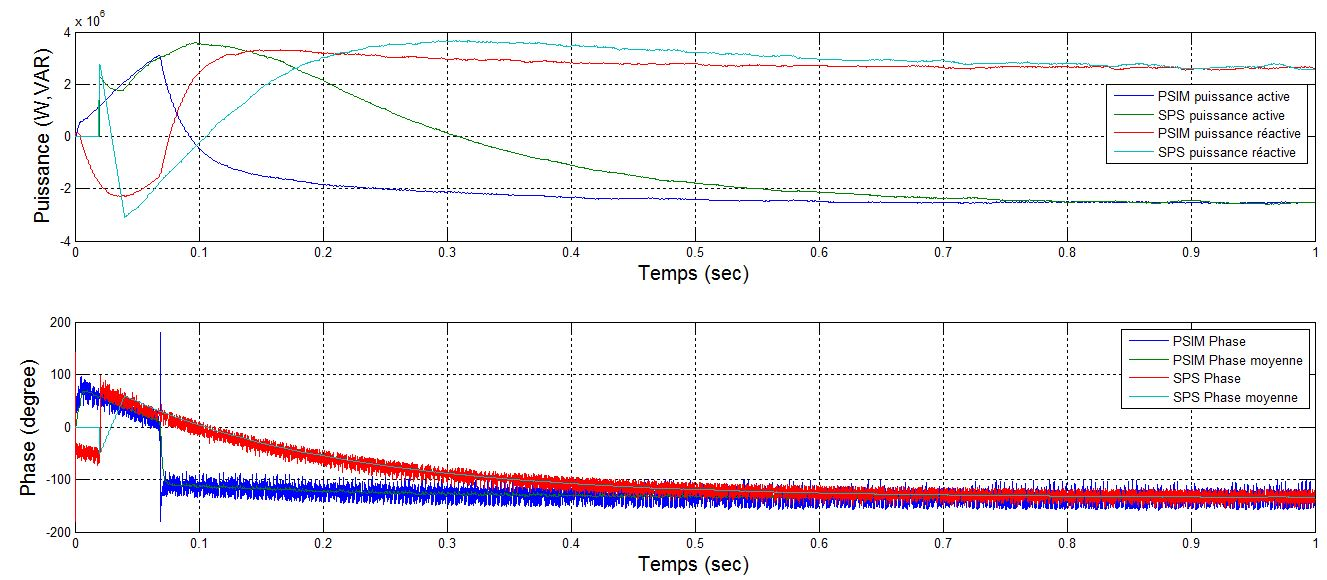
\includegraphics[scale=0.5]{fig/AFEIDEAL/pui_135.jpg}}
\caption{Puissances active et réactive pour une courant déphasé de -135$^\circ$, pour un pas de calcul 1$\mu$s}
\label{AF_I_pui__135}
\end{figure}


\clearpage

\subsection{Analyse des résultats comparatifs de SPS et de PSIM pour un pas de calcul de 1$\mu$s}
La figure \ref{AF_I_cou} présente le courant à l'entrée du redresseur. On remarque que les patrons de courants sont similaires, mais qu'il existe un léger décalage entre les 2 simulations. Il existe des différences notables dans l'onde lorsque celle-ci est autour d'une valeur angulaire de ($\pi/2$), si l'on suppose un sinus. Cette différence ainsi que le décalage s'expliquent par l'implantation de la fonction d'hystérésis qui n'est pas identique dans les 2 simulateurs. On note que les fonctions non-linéaires comme la fonction de seuillage par hystérésis sont sensibles aux méthodes de calculs et aux particularités des simulateurs. On peut le constater par la figure du courant d'entrée.

Ls figure \ref{AF_I_pui_45} présente la puissance active et réactive mesurée dans les 2 simulateurs pour une valeur d'angle imposée de 45$^\circ$ de déphasage du courant par rapport à la tension. On note rapidement que la lecture n'est précise qu'à partir d'un nombre important de cycles, l'initialisation du calcul étant intrinsèquement liée aux méthodes de simulation jumelée à l'implantation du bloc dans le simulateur. La mesure de puissance implique des transformations fréquentielles ainsi que des filtres qui réduisent la dynamique du système. Les filtres employés sont sensibles au pas de calcul et peuvent présenter des différences entre les simulateurs. On note que les mesures sont lentes comparé au procédé.

Les figures \ref{AF_I_pui_135}, \ref{AF_I_pui__45} et \ref{AF_I_pui__135} présentent la puissance active et réactive sur les 2 simulateurs pour des valeurs de déphasage de courant qui sont de 135$^\circ$, -45$^\circ$ et -135$^\circ$. Les constatations sont analogues à celles effectuées précédemment. Ces résultats montrent le fonctionnement 4 quadrants de l'AFE sur source idéale avec régulation de courant côté source et permettent de constater l'usage d'un tel dispositif, soit d'imposer le facteur de puissance vu de la source. 
\section{AFE 2 niveaux avec contrôle par hystérésis débitant sur une charge RC}
Le modèle de redresseur 2 niveaux AFE avec contrôle par hystérésis débitant sur une charge RC est le même que celui présenté à la section précédente. Le circuit du convertisseur est présenté à la figure \ref{circuit_AFE_2L_RC}. La source idéale du montage précédent est remplacée par une charge RC, composée d'une résistance de 9.26$\Omega$ et d'un condensateur initialement chargé à 5000V, d'une capacité de 330mF. La résistance de 9.26$\Omega$ est calculée selon l'approximation suivante:

\begin{equation}
R_{eq} = \frac{V_{CC}^2}{P_{moy}} = \frac{5000^2}{2.7 \times 10^6} = 9.26\Omega
\end{equation}
De plus, contrairement au montage précédent, il n'y a plus de rétroaction sur l'angle du courant. L'angle de la référence de courant est en phase avec la tension du réseau (pour un fonctionnement à facteur unitaire). La figure \ref{fft_RC} représente le calcul de transformée de Fourier discrète (fft) d'une phase du courant d'entrée. Les paramètres de l'hystérésis ont été ajustés afin que la fréquence de commutation (qui glisse avec cette méthode de commande), soit près de 1kHz. Le tableau \ref{p_AF_RC} présente les paramètres utilisés pour l'AFE 2 niveaux débitant sur une charge RC.

\begin{figure}[htb]
\makebox[\textwidth][c]{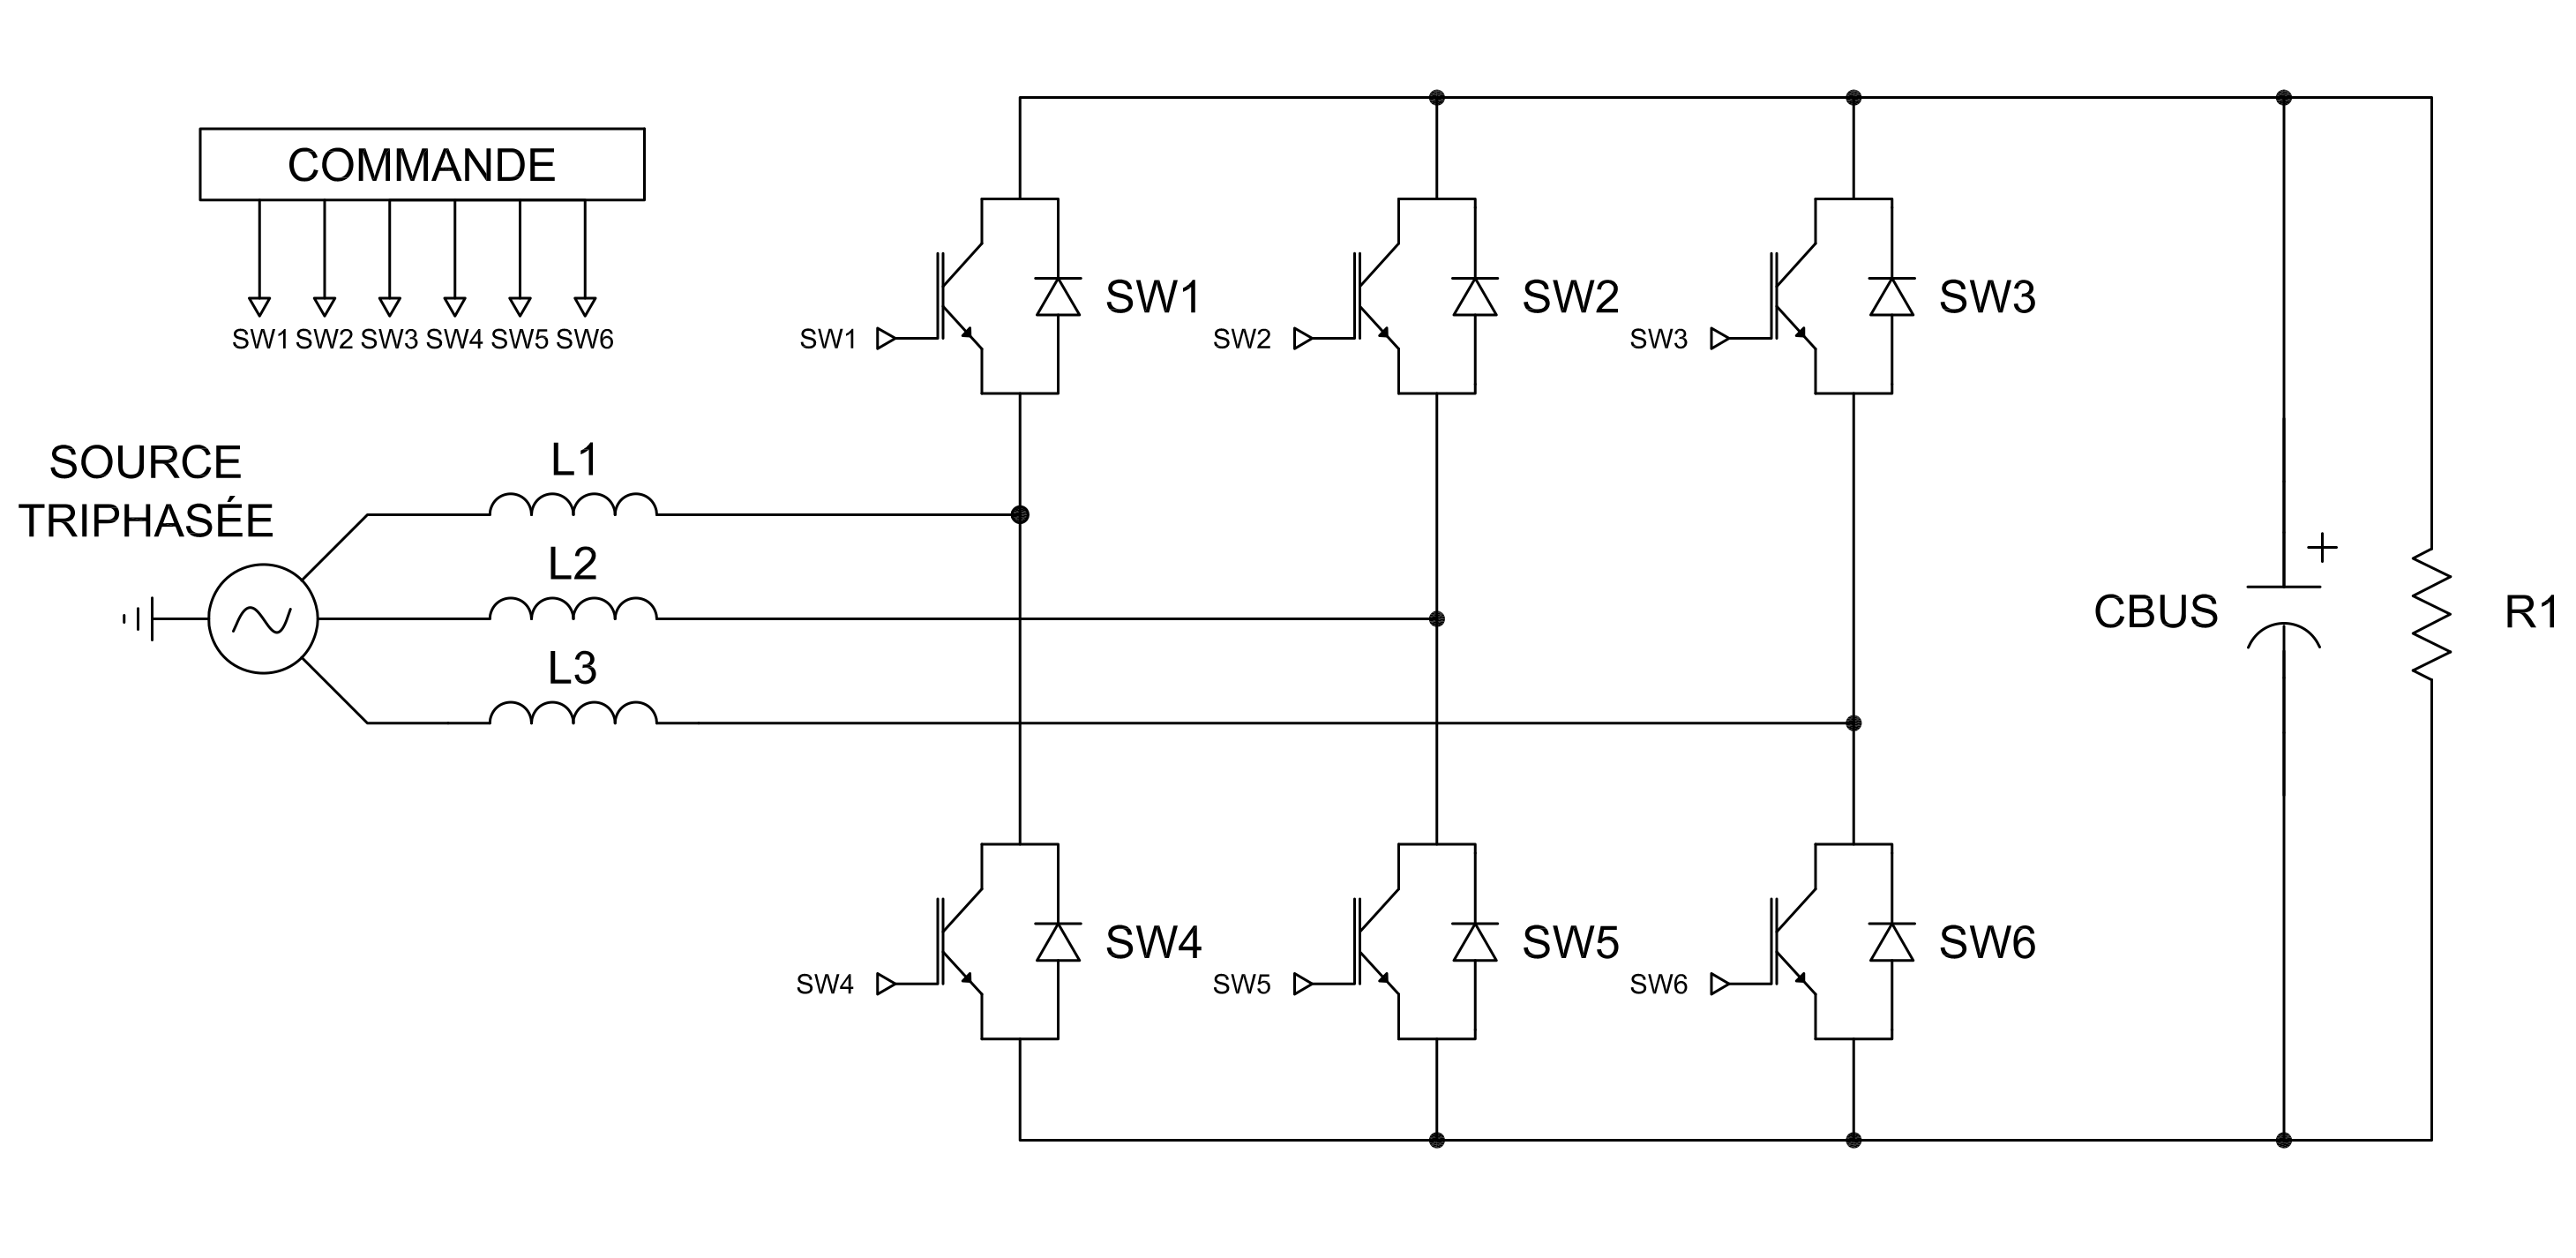
\includegraphics[scale=0.6]{fig/AFE_2L_RC.png}}
\caption{Circuit électrique de l'AFE 2 niveaux sur une charge RC}
\label{circuit_AFE_2L_RC}
\end{figure}


\begin{figure}[htb]
\makebox[\textwidth][c]{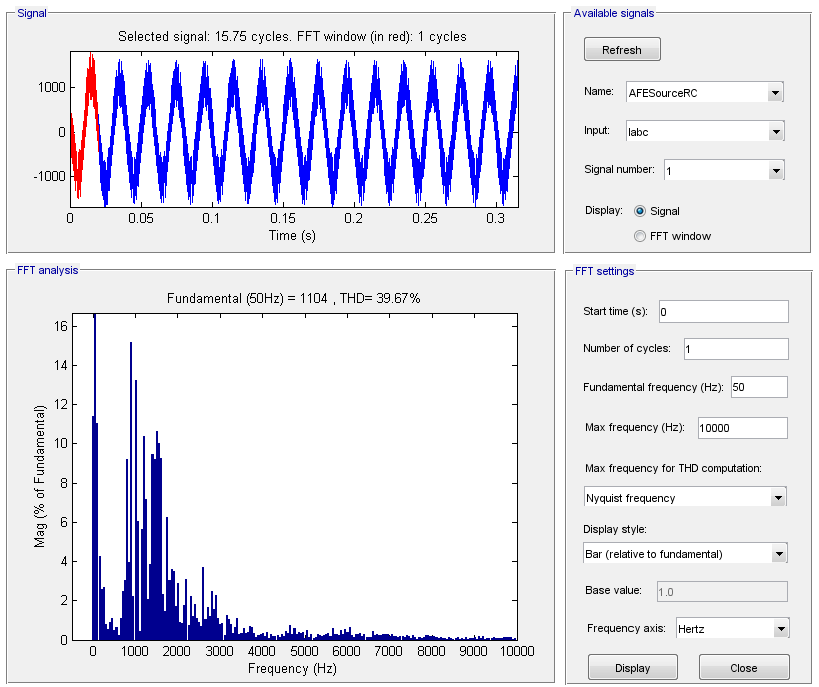
\includegraphics[scale=0.5]{fig/AFERC/FFTAnalysisToolResult5u.png}}
\caption{La transformée de Fourier discrète (fft) du courant d'entrée à 1$\mu$s}
\label{fft_RC}
\end{figure}


\begin{table}[htb]
\centering
\begin{tabular}{|l|c|} 
  \hline
  \textbf{Paramètre} & \textbf{Valeur}  \\
  \hline\hline
  Tension de référence CC & 5000 V\\ \hline
  Seuil hystérésis & 450 A\\ \hline
  Inductance côté AC& 814.87 $\mu$H\\ \hline
  Courant maximal à l'entrée& 1500 A \\ \hline \hline
  \multicolumn{2}{|l|}{\textbf{IGBT}}\\ \hline
  Résistance interne & 0.001 $\Omega$\\
  Résistance du snubber & 100k $\Omega$\\ \hline \hline
   \multicolumn{2}{|l|}{\textbf{PI courant}}\\ \hline
  Gain proportionnel & 150 \\
  Gain intégrateur & 1.2e4 \\ \hline \hline
  \multicolumn{2}{|l|}{\textbf{Charge}}\\ \hline
  Résistance & 9.26 $\Omega$ \\
  Capacité d'entrée & 330 mF\\
  \hline
\end{tabular}
\caption{Paramètres de simulation pour l'AFE 2 niveaux avec contrôle par hystérésis débitant sur charge RC}
\label{p_AF_RC}
\end{table}

\clearpage

\subsection{Résultats de simulation pour SPS et PSIM pour un pas de calcul de 1$\mu$s}
Cette section présente les résultats de simulation de l'AFE 2 niveaux avec contrôle pas hystérésis sur charge RC, pour un pas de calcul discret de 1$\mu$s. 




\begin{figure}[htb]
\makebox[\textwidth][c]{\includegraphics[scale=0.5]{fig/AFERC/cour_al.jpg}}
\caption{Le courant d'entré à 1$\mu$s pour l'AFE sur charge RC}
\label{AF_RC_cou}
\end{figure}




\begin{figure}[htb]
\makebox[\textwidth][c]{\includegraphics[scale=0.5]{fig/AFERC/vch.jpg}}
\caption{La tension à la charge à 1$\mu$s pour l'AFE sur charge RC}
\label{AF_RC_ten}
\end{figure}



\begin{figure}[htb]
\makebox[\textwidth][c]{\includegraphics[scale=0.5]{fig/AFERC/IGBT.jpg}}
\caption{La tension et le courant au bornes d'un IGBT à 1$\mu$s pour l'AFE sur charge RC}
\label{AF_RC_igbt}
\end{figure}

\clearpage

\subsection{Analyse des résultats comparatifs de SPS et de PSIM pour un pas de calcul de 1$\mu$s}

La figure \ref{AF_RC_cou} présente le courant à l'entrée de l'AFE pour les 2 simulateurs. Tout comme dans la section précédente, force est de constater que le comportement de l'hystérésis a un impact sur la qualité de l'onde dans PSIM. On remarque que le comportement dans SPS est plus régulier et permet d'obtenir un fonctionnement plus réaliste et potentiellement un glissement de fréquence de commutation (dispersion harmonique) plus faible. Les niveaux d'amplitudes sont différents en raison des surtensions dans PSIM. Le déphasage des fondamentales est moins important que dans la simulation précédente, en raison de l'absence de la régulation d'angle. 

La figure \ref{AF_RC_ten} présente la tension du bus CC en fonction du temps pour un condensateur initialement chargé. Le but est d'observer la dynamique de régulation de l'AFE. On constate que les différences sont faibles et que les 2 simulateurs fournissent un résultat similaire, malgré que le courant d'entrée soit différent.

La figure \ref{AF_RC_igbt} présente la tension et le courant d'un IGBT de l'AFE dans les 2 simulateurs. On remarque que la tension des IGBT présente des différences importantes, que l'on attribue au comportement de l'hystérésis qui détermine les temps de conduction. La forme d'onde de tension explique ce qui est observé sur l'onde de courant à l'entrée de l'AFE. Il en est de même pour l'onde de courant qui montre une plus grande régularité dans SPS.


\section{AFE 3 niveaux NPC avec contrôle par MLI}
L'AFE 3 niveaux NPC avec contrôle par MLI est composé de 12 interrupteurs IGBT ainsi que de 6 diodes de point milieu. Il représente la version finale du sous-système de l'AFE. La méthode de commande implantée diffère de celle implantée au CERN qui utilise une transformation de Park afin de simplifier le contrôle. La méthode employée pour la validation croisée est une méthode de régulation qui module directement le courant à 50Hz, sans transformation intermédiaire. Le modèle dq a été implanté pour prototypage dans le simulateur final. Le circuit électrique de l'AFE 3 niveaux sur charge RC est présenté à la figure \ref{circuit_AFE_3L_RC}. Le tableau \ref{p_AF_3level} présente les paramètres utilisés avec l'AFE 3 niveaux NPC.


\begin{table}[htb]
\centering
\begin{tabular}{|l|c|} 
  \hline
  \textbf{Paramètre} & \textbf{Valeur}  \\
  \hline\hline
  Tension référence CC & 5000 V\\ \hline
  Fréquence de modulation & 1000 Hz \\ \hline
  Inductance côté AC& 814.87 $\mu$H\\ \hline
  Courant maximal à l'entrée& 800 A \\ \hline \hline
  \multicolumn{2}{|l|}{\textbf{IGBT}}\\ \hline
  Résistance interne & 0.001 $\Omega$\\
  Résistance du snubber & 100k $\Omega$\\ \hline \hline
   \multicolumn{2}{|l|}{\textbf{PI courant}}\\ \hline
  Gain proportionnel & 282.9218 \\
  Gain intégrateur & 92.59 \\ \hline \hline
  \multicolumn{2}{|l|}{\textbf{PI commande}}\\ \hline
  Rapport cyclique maximal & 0.95\\
  Gain proportionnel & 7.5e-4 \\
  Gain intégrateur & 0.005 \\ \hline \hline
  \multicolumn{2}{|l|}{\textbf{Charge}}\\ \hline
  Résistance & 9.26 $\Omega$ \\
  Capacité d'entrée & 330 mF\\
  \hline
\end{tabular}
\caption{Paramètres de simulation pour l'AFE 3 niveaux NPC avec contrôle par MLI}
\label{p_AF_3level}
\end{table}

\begin{figure}[htb]
\makebox[\textwidth][c]{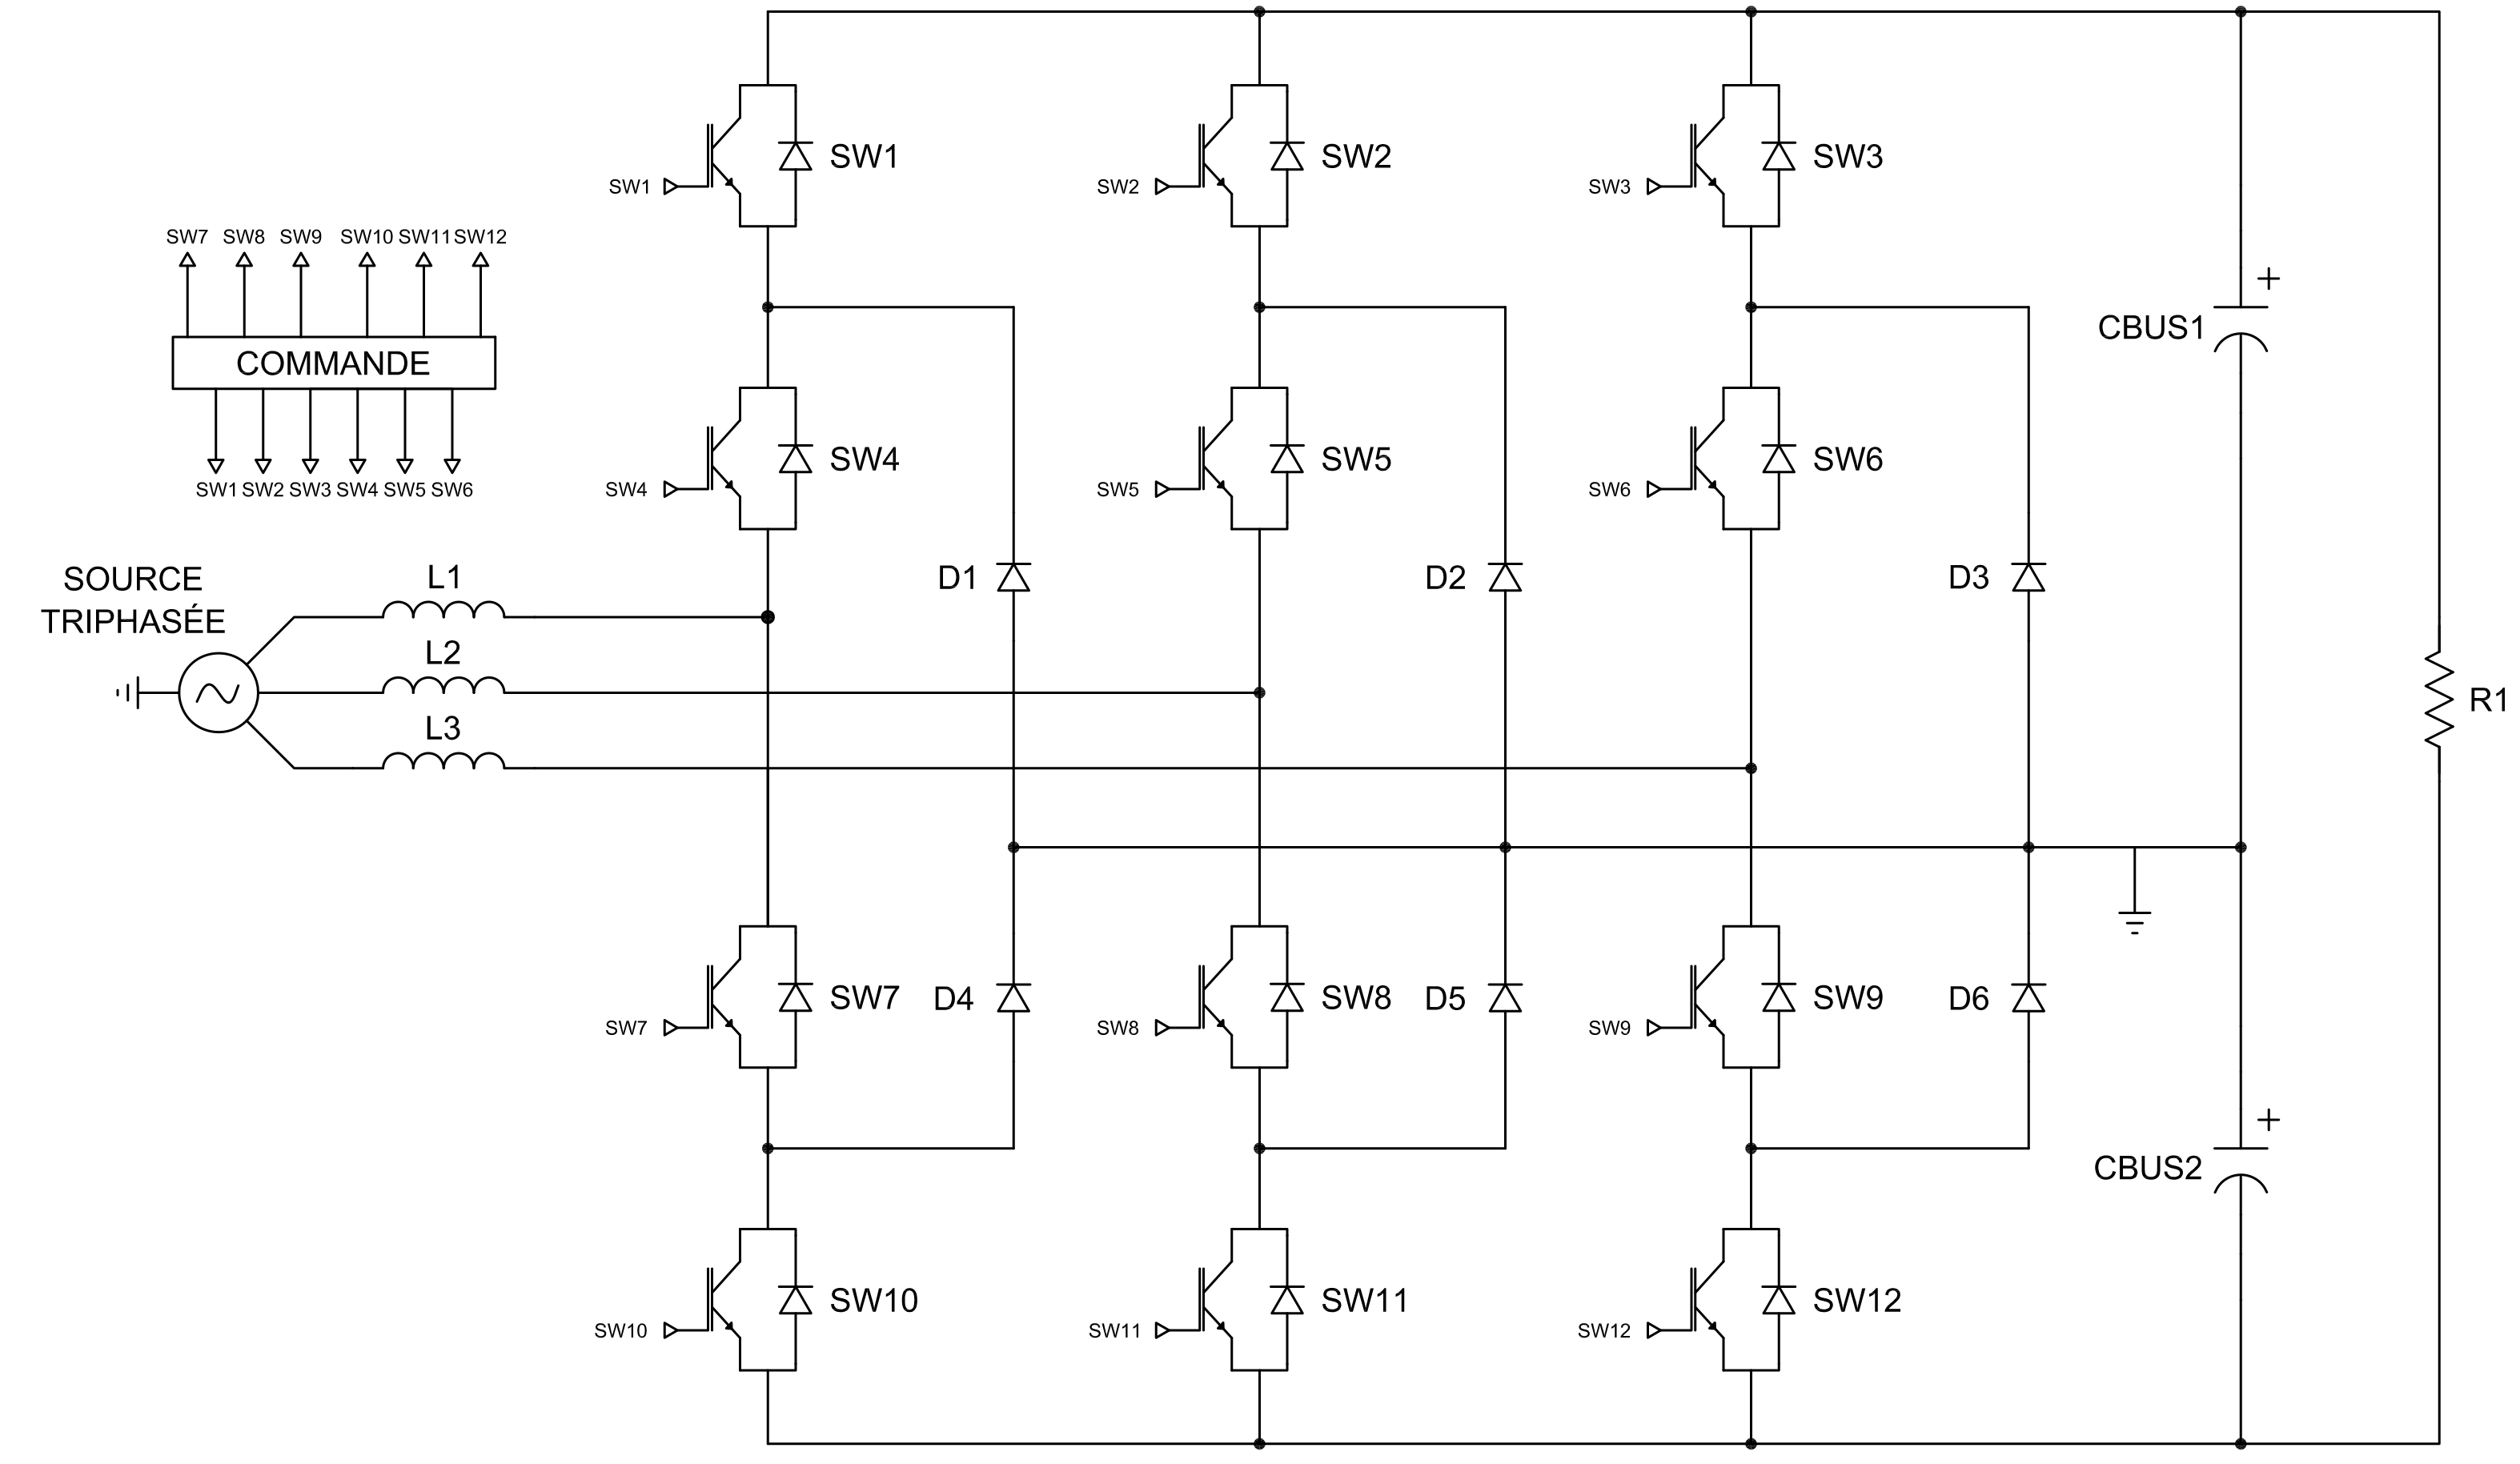
\includegraphics[scale=0.6]{fig/AFE_3L_RC.png}}
\caption{Circuit électrique de l'AFE 3 niveaux sur charge RC}
\label{circuit_AFE_3L_RC}
\end{figure}


\clearpage


\subsection{Résultats de simulation pour SPS et PSIM pour un pas de calcul de 1$\mu$s}
Cette section présente les courbes d'intérêt pour la simulation de l'AFE 3 niveaux NPC avec contrôle par MLI, pour un pas de 1$\mu$s. 

\begin{figure}[htb]
\makebox[\textwidth][c]{\includegraphics[scale=0.5]{fig/AFE3LEVEL/1u/cour_al.jpg}}
\caption{Le courant d'entrée pour un pas de calcul de 1$\mu$s, pour l'AFE 3 niveaux}
\label{AF_3_cou}
\end{figure}


\begin{figure}[htb]
\makebox[\textwidth][c]{\includegraphics[scale=0.5]{fig/AFE3LEVEL/1u/vch.jpg}}
\caption{La tension à la charge pour un pas de calcul de 1$\mu$s, pour l'AFE 3 niveaux}
\label{AF_3_vch}
\end{figure}


\begin{figure}[htb]
\makebox[\textwidth][c]{\includegraphics[scale=0.5]{fig/AFE3LEVEL/1u/IGBT.jpg}}
\caption{La tension et le courant au niveau d'un IGBT pour un pas de calcul de 1$\mu$s, pour l'AFE 3 niveaux}
\label{AF_3_IGBT}
\end{figure}

\begin{figure}[htb]
\makebox[\textwidth][c]{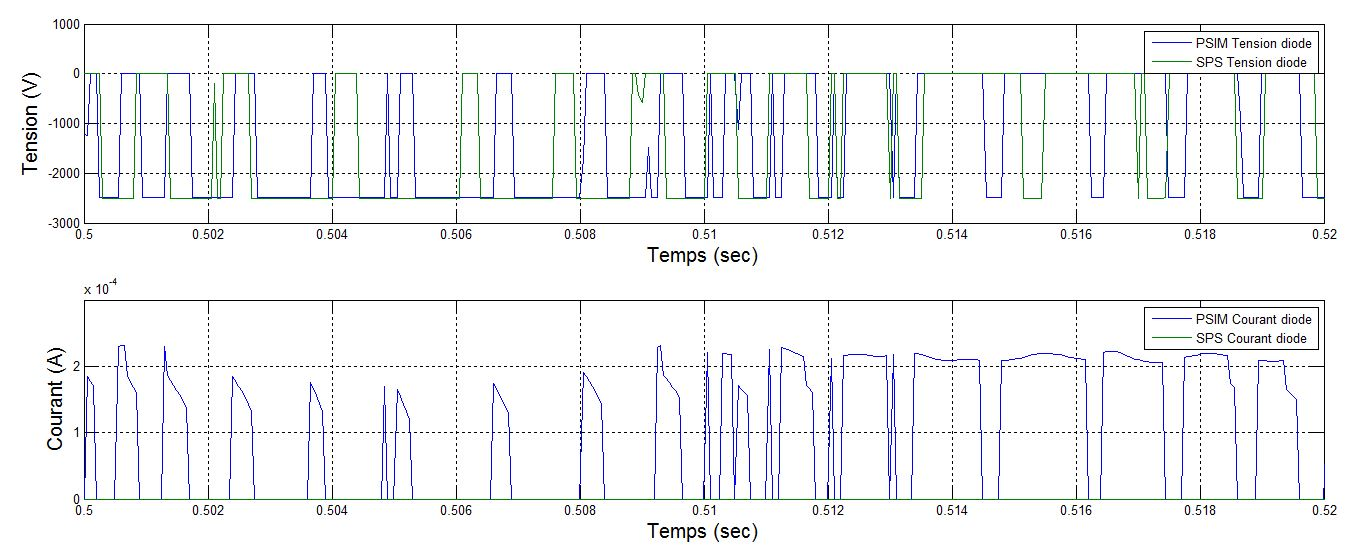
\includegraphics[scale=0.5]{fig/AFE3LEVEL/1u/DIODE.jpg}}
\caption{La tension et le courant au niveau d'une diode pour un pas de calcul de 1$\mu$s, pour l'AFE 3 niveaux}
\label{AF_3_DIODE}
\end{figure}


\clearpage

\subsection{Analyse des résultats comparatifs de SPS et de PSIM pour un pas de calcul de 1$\mu$s}
La figure \ref{AF_3_cou} présente le courant d'entrée de l'AFE 3 niveaux avec contrôle par MLI. Contrairement au contrôle par hystérésis, le contrôle par MLI offre un fonctionnement beaucoup plus stable dans les 2 simulateurs. Les courbes sont pratiquement indissociables. Cela signifie que la dynamique d'implantation des PI est pratiquement identique pour les 2 simulateurs.

La figure \ref{AF_3_vch} présente la tension à la charge pour le redresseur 3 niveaux. On remarque que l'ondulation de tension est beaucoup plus faible et que les courbes sont indissociables. 

La figure \ref{AF_3_IGBT} présente la tension et le courant dans l'un des IGBT de l'AFE 3 niveaux. Contrairement à l'AFE 2 niveaux par hystérésis, on remarque une superposition des courbes et des décalages beaucoup plus faibles. Les erreurs sont minimes et causées par la détection de passage par 0 qui varie suivant la méthode de solution (équations d'états ou matrice d'admittances) ainsi que selon l'algorithme de détection de passage par 0 (Tustin ou trapézoïdal pur).

La figure \ref{AF_3_DIODE} présente la tension et le courant dans l'une des diodes de point milieu de l'AFE 3 niveaux. La tension aux bornes des diodes montre qu'elles s'amorcent aux mêmes instants. Les constats sont les mêmes que ceux des IGBT sur les sources d'erreur. 
\section{AFE 2 niveaux avec contrôle par hystérésis et hacheur 4 quadrants à 4 IGBT}
Cette section présente les résultats de simulations obtenus sur PSIM et SPS pour l'AFE 2 niveaux avec contrôle par hystérésis et hacheur 4 quadrants à 4 IGBT. Le circuit électronique des 2 convertisseurs est présenté à la figure \ref{circuit_H4Q_AFE_2L_RC}. Le tableau \ref{p_AF_hash} présente les paramètres utilisés dans les simulations.

\begin{figure}[htb]
\makebox[\textwidth][c]{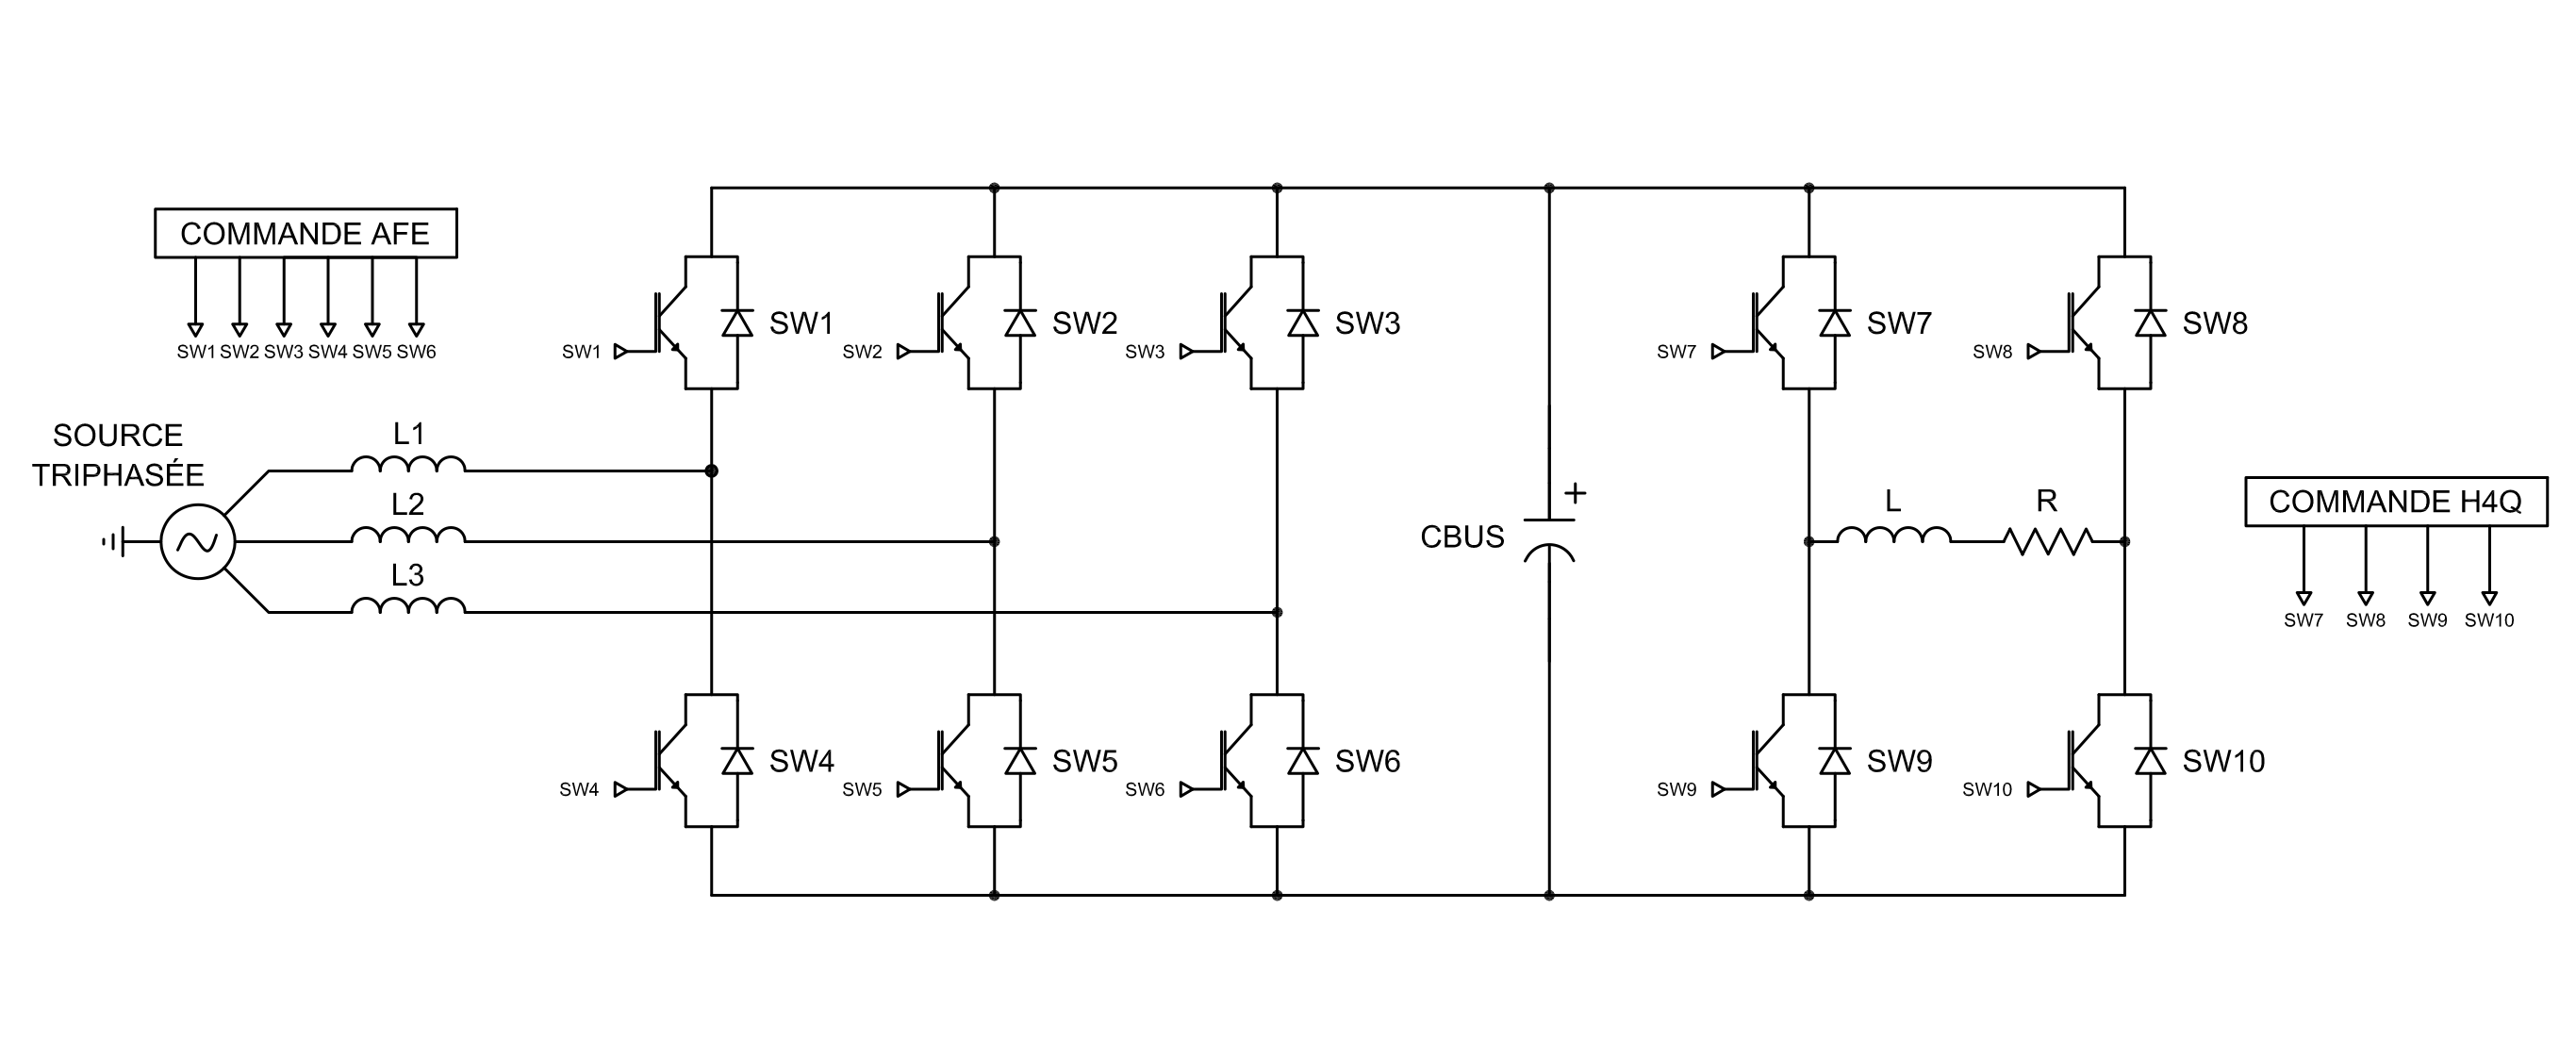
\includegraphics[scale=0.6]{fig/H4Q_AFE_2L_RC.png}}
\caption{Circuit électrique de l'AFE 2 niveaux avec contrôle par hystérésis et hacheur 4 quadrants à 4 IGBT}
\label{circuit_H4Q_AFE_2L_RC}
\end{figure}


\begin{table}[htb]
\centering
\begin{tabular}{|l|c|} 
  \hline
  \textbf{Paramètre} & \textbf{Valeur}  \\
  \hline\hline \hline
  \multicolumn{2}{|l|}{\textbf{AFE 2 niveaux}}\\ \hline \hline 
  Tension référence CC & 5000 V\\ \hline
  Seuil hystérésis & 450A\\ \hline
  Inductance côté AC& 814.87 $\mu$H\\ \hline
  Courant maximal à l'entrée& 1500A \\ \hline \hline
  \multicolumn{2}{|l|}{\textbf{IGBT AFE}}\\ \hline
  Résistance interne & 0.001 $\Omega$\\
  Résistance du snubber & 100k $\Omega$\\ \hline \hline
   \multicolumn{2}{|l|}{\textbf{PI courant AFE}}\\ \hline
  Gain proportionnel & 150 \\
  Gain intégrateur & 1.2e4 \\ \hline \hline
  \multicolumn{2}{|l|}{\textbf{Bus CC}}\\ \hline
  Capacité d'entrée & 330 mF\\
  \hline \hline \hline
  
  \multicolumn{2}{|l|}{\textbf{Hacheur 4 quadrants}}\\ \hline \hline
  Fréquence de modulation & 1000 Hz\\ \hline
  Rapport cyclique maximal & 0.95 \\ \hline \hline
  \multicolumn{2}{|l|}{\textbf{IGBT hacheur}}\\ \hline
  Résistance interne & 0.001 $\Omega$\\
  Résistance du snubber & 100k $\Omega$\\ \hline \hline
   \multicolumn{2}{|l|}{\textbf{PI hacheur}}\\ \hline
  Gain proportionnel & 0.071 \\
  Gain intégrateur & 50 \\ \hline \hline
  \multicolumn{2}{|l|}{\textbf{Charge}}\\ \hline
  Résistance & 0.28 $\Omega$\\
  Inductance & 0.1 H\\
  \hline
\end{tabular}
\caption{Paramètres de simulation pour l'hacheur 4 quadrants à 4 interrupteurs avec l'AFE 2 niveaux}
\label{p_AF_hash}
\end{table}
\clearpage

\subsection{Résultats de simulation pour SPS et PSIM pour un pas de calcul de 1$\mu$s}
Cette section présente les résultats de simulation pour l'hacheur 4 quadrants à 4 interrupteurs avec l'AFE 2 niveaux sur PSIM et sur SPS, pour un pas de calcul discret de 1$\mu$s. 


\begin{figure}[htb]
\makebox[\textwidth][c]{\includegraphics[scale=0.5]{fig/Hach_AFE/1u/cour_al.jpg}}
\caption{Courant d'entrée pour un pas de calcul de 1$\mu$s pour la section AFE}
\label{AF_HA_cou1}
\end{figure}


\begin{figure}[htb]
\makebox[\textwidth][c]{\includegraphics[scale=0.5]{fig/Hach_AFE/1u/ten_bus.jpg}}
\caption{La tension au bus CC à 1$\mu$s section AFE}
\label{AF_HA_vch1}
\end{figure}



\begin{figure}[htb]
\makebox[\textwidth][c]{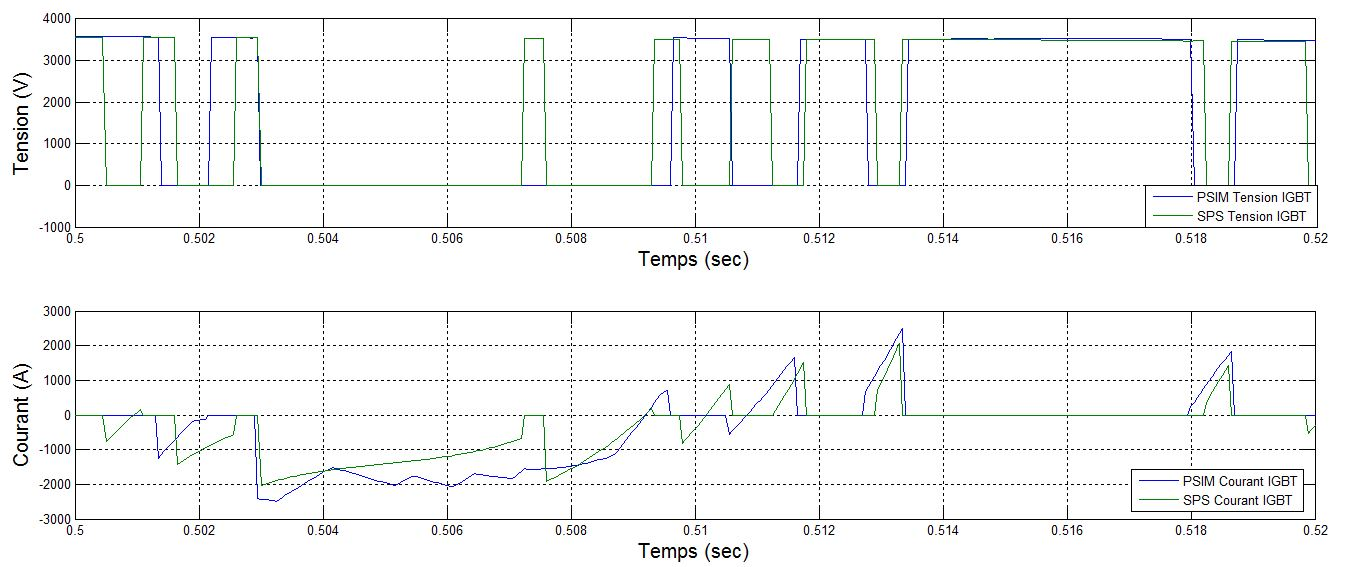
\includegraphics[scale=0.5]{fig/Hach_AFE/1u/IGBT_AFE.jpg}}
\caption{La tension et le courant au niveau d'un IGBT à 1$\mu$s au niveau de l'AFE}
\label{AF_HA_IGBT1}
\end{figure}


\begin{figure}[htb]
\makebox[\textwidth][c]{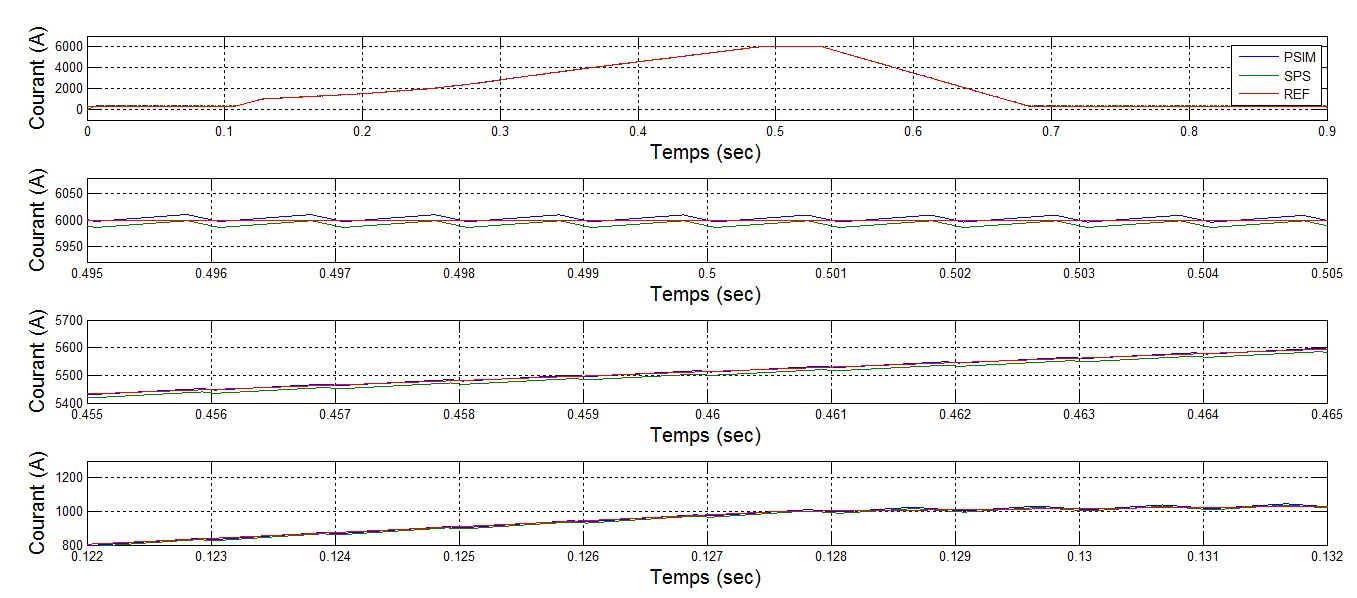
\includegraphics[scale=0.5]{fig/Hach_AFE/1u/hach_cou_ch.jpg}}
\caption{Le courant au niveau de la charge à 1$\mu$s}
\label{AF_HA_CHA1}
\end{figure}



\begin{figure}[htb]
\makebox[\textwidth][c]{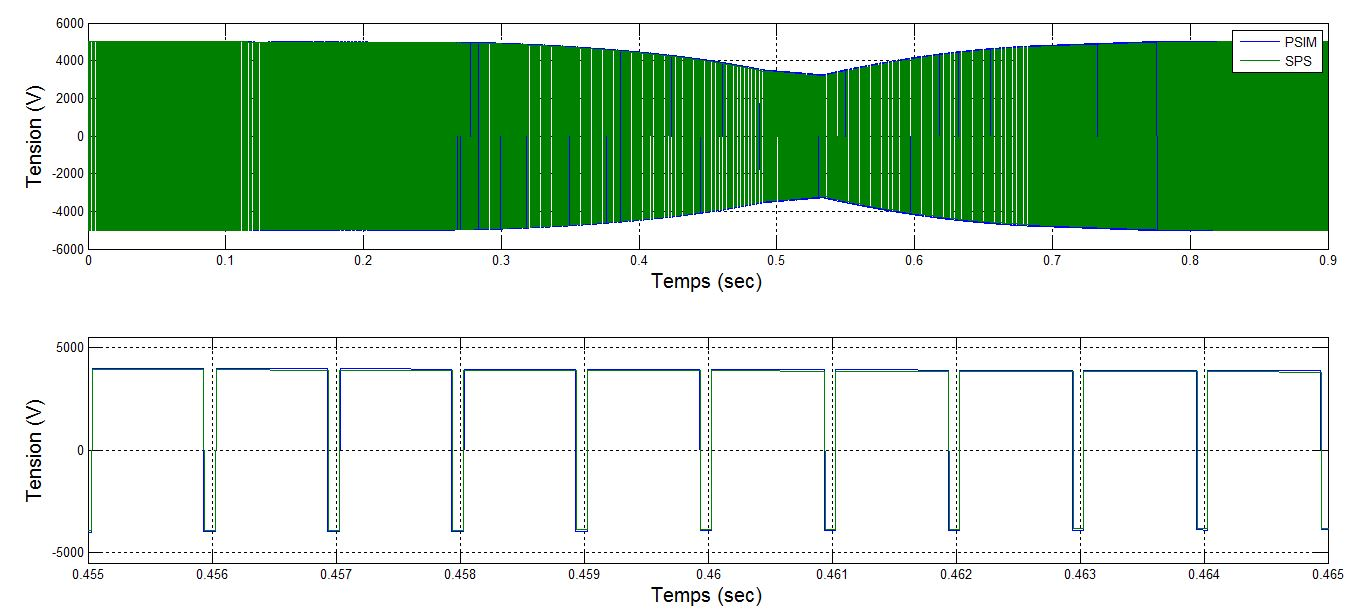
\includegraphics[scale=0.5]{fig/Hach_AFE/1u/hach_ten_ch.jpg}}
\caption{La tension au niveau de la charge à 1$\mu$s}
\label{AF_HA_CHV1}
\end{figure}

\begin{figure}[htb]
\makebox[\textwidth][c]{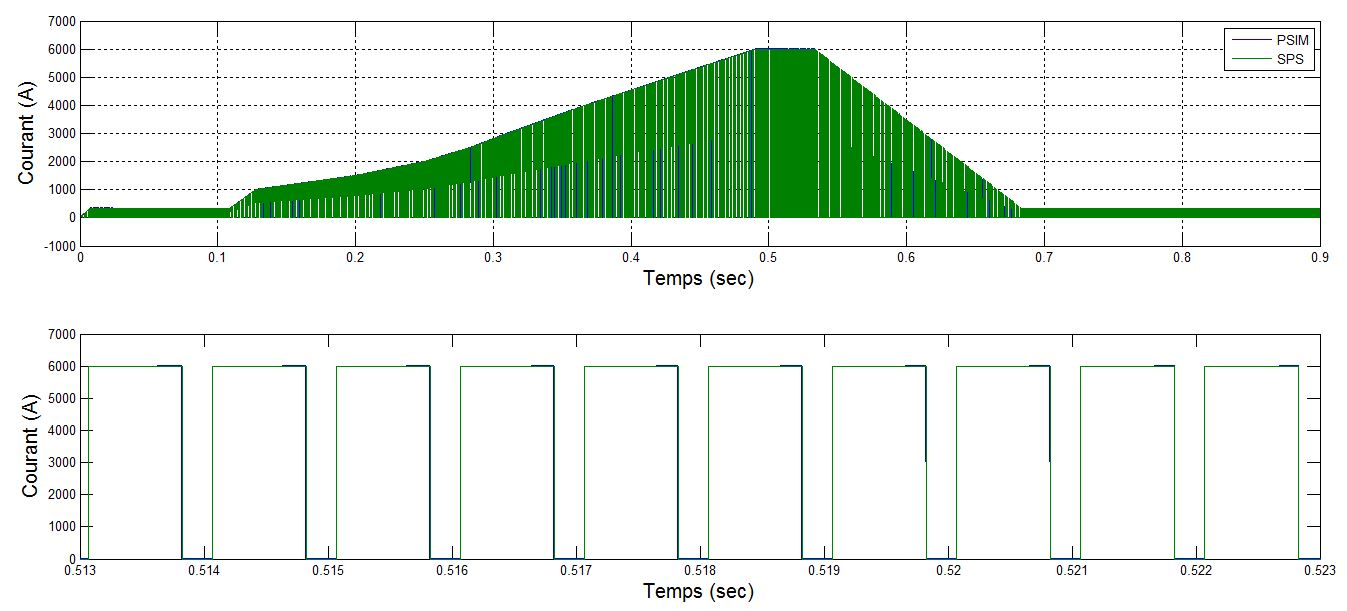
\includegraphics[scale=0.5]{fig/Hach_AFE/1u/IGBT_cou_hach.jpg}}
\caption{Le courant aux bornes d'un IGBT à 1$\mu$s pour le hacheur 4 quadrants}
\label{AF_HA_HAA1}
\end{figure}

\begin{figure}[htb]
\makebox[\textwidth][c]{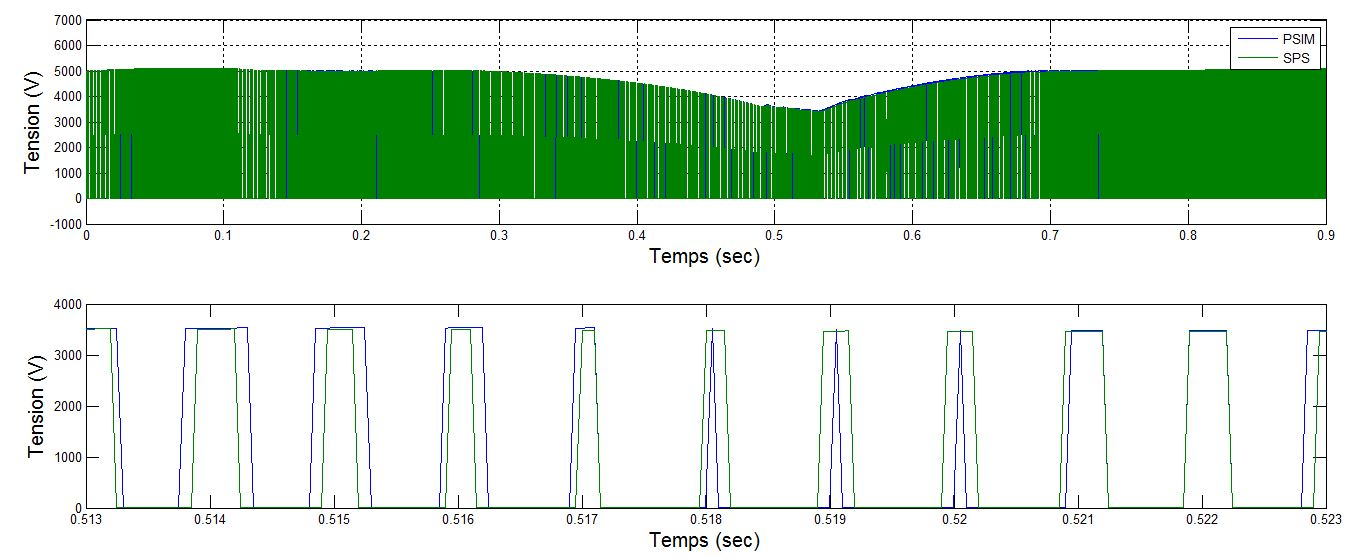
\includegraphics[scale=0.5]{fig/Hach_AFE/1u/IGBT_ten_hach.jpg}}
\caption{La tension aux bornes d'un IGBT à 1$\mu$s pour le hacheur 4 quadrants}
\label{AF_HA_HAV1}
\end{figure}



\clearpage

\subsection{Analyse des résultats comparatifs de SPS et de PSIM pour un pas de calcul de 1$\mu$s}

La figure \ref{AF_HA_cou1} présente le courant d'entrée de l'AFE 2 niveaux avec contrôle par hystérésis. On remarque premièrement que les signaux sont en phase et que les amplitudes sont identiques. Cependant, l'impact des commutations sur la forme de courant diffère d'une simulation à l'autre pour les mêmes raisons qu'énoncées à la section portant sur l'AFE 2 niveaux avec contrôle par hystérésis sur charge RC. Les signaux présentent un faible déphasage, mais l'impact des commutations est plus marqué dans SPS que dans PSIM.

La figure \ref{AF_DC_vch1} présente la tension du bus CC en fonction du temps pour un cycle d'alimentation des électroaimants. On remarque que les courbes ont exactement la même forme, mais qu'il y a un facteur d'échelle allant jusqu'à 200V entre les courbes. Le fonctionnement du hacheur 4 quadrants à 4 IGBT ne présentant pas de différences par rapport à celui analysé précédemment, tel qu'on peut l'observer aux figures \ref{AF_HA_CHA1} et \ref{AF_HA_CHV1}. Les erreurs entre les simulations sont pratiquement négligeables à cet effet. Les figures \ref{AF_HA_HAA1} et \ref{AF_HA_HAV1} présentent respectivement le courant et la tension d'un IGBT du hacheur 4 quadrants. Les différences sont pratiquement invisibles. Comme il a déjà été statué que les contrôleurs possédaient la même dynamique selon les simulateurs, il ne reste que les blocs d'hystérésis qui peuvent occasionner des différences, tel que noté pour l'AFE. La forme d'onde de courant étant différente, on se doute que la puissance instantanée est différente et qu'en contrôle dynamique, les erreurs sont cumulatives. Les hypothèses peuvent être confirmées par le courant et la tension des IGBT de l'AFE, présentée à la figure \ref{AF_HA_IGBT1}. On voit clairement les différences entre les formes de tension et de courant, ce qui confirme qu'ils ne conduisent pas aux mêmes moments. Cependant, à la figure \ref{AF_HA_HAA1} ainsi qu'à la figure \ref{AF_HA_HAV1} on constate que les interrupteurs du hacheur conduisent au mêmes moments. La preuve est donc faite que la source d'erreur apparente est inhérente aux modèles d'interrupteurs et est reliée à l'implantation de l'hystérésis du côté de l'AFE. 

\section{AFE 3 niveaux NPC avec contrôle par MLI avec convertisseur CC-CC formé de 2 cellules NPC 3 niveaux}
Cette section présente les résultats de simulations obtenus sur PSIM et sur SPS pour le système complet, formé d'un redresseur AFE 3 niveaux avec régulation MLI et d'un convertisseur CC-CC composé de 2 cellules NPC 3 niveaux.  Le circuit électronique du système complet est présenté à la figure \ref{circuit_AFE_3L_RC_DCP_DCN}. Le tableau \ref{p_AF_DCP} présente les paramètres utilisés dans les sous-systèmes.

\begin{figure}[htb]
\makebox[\textwidth][c]{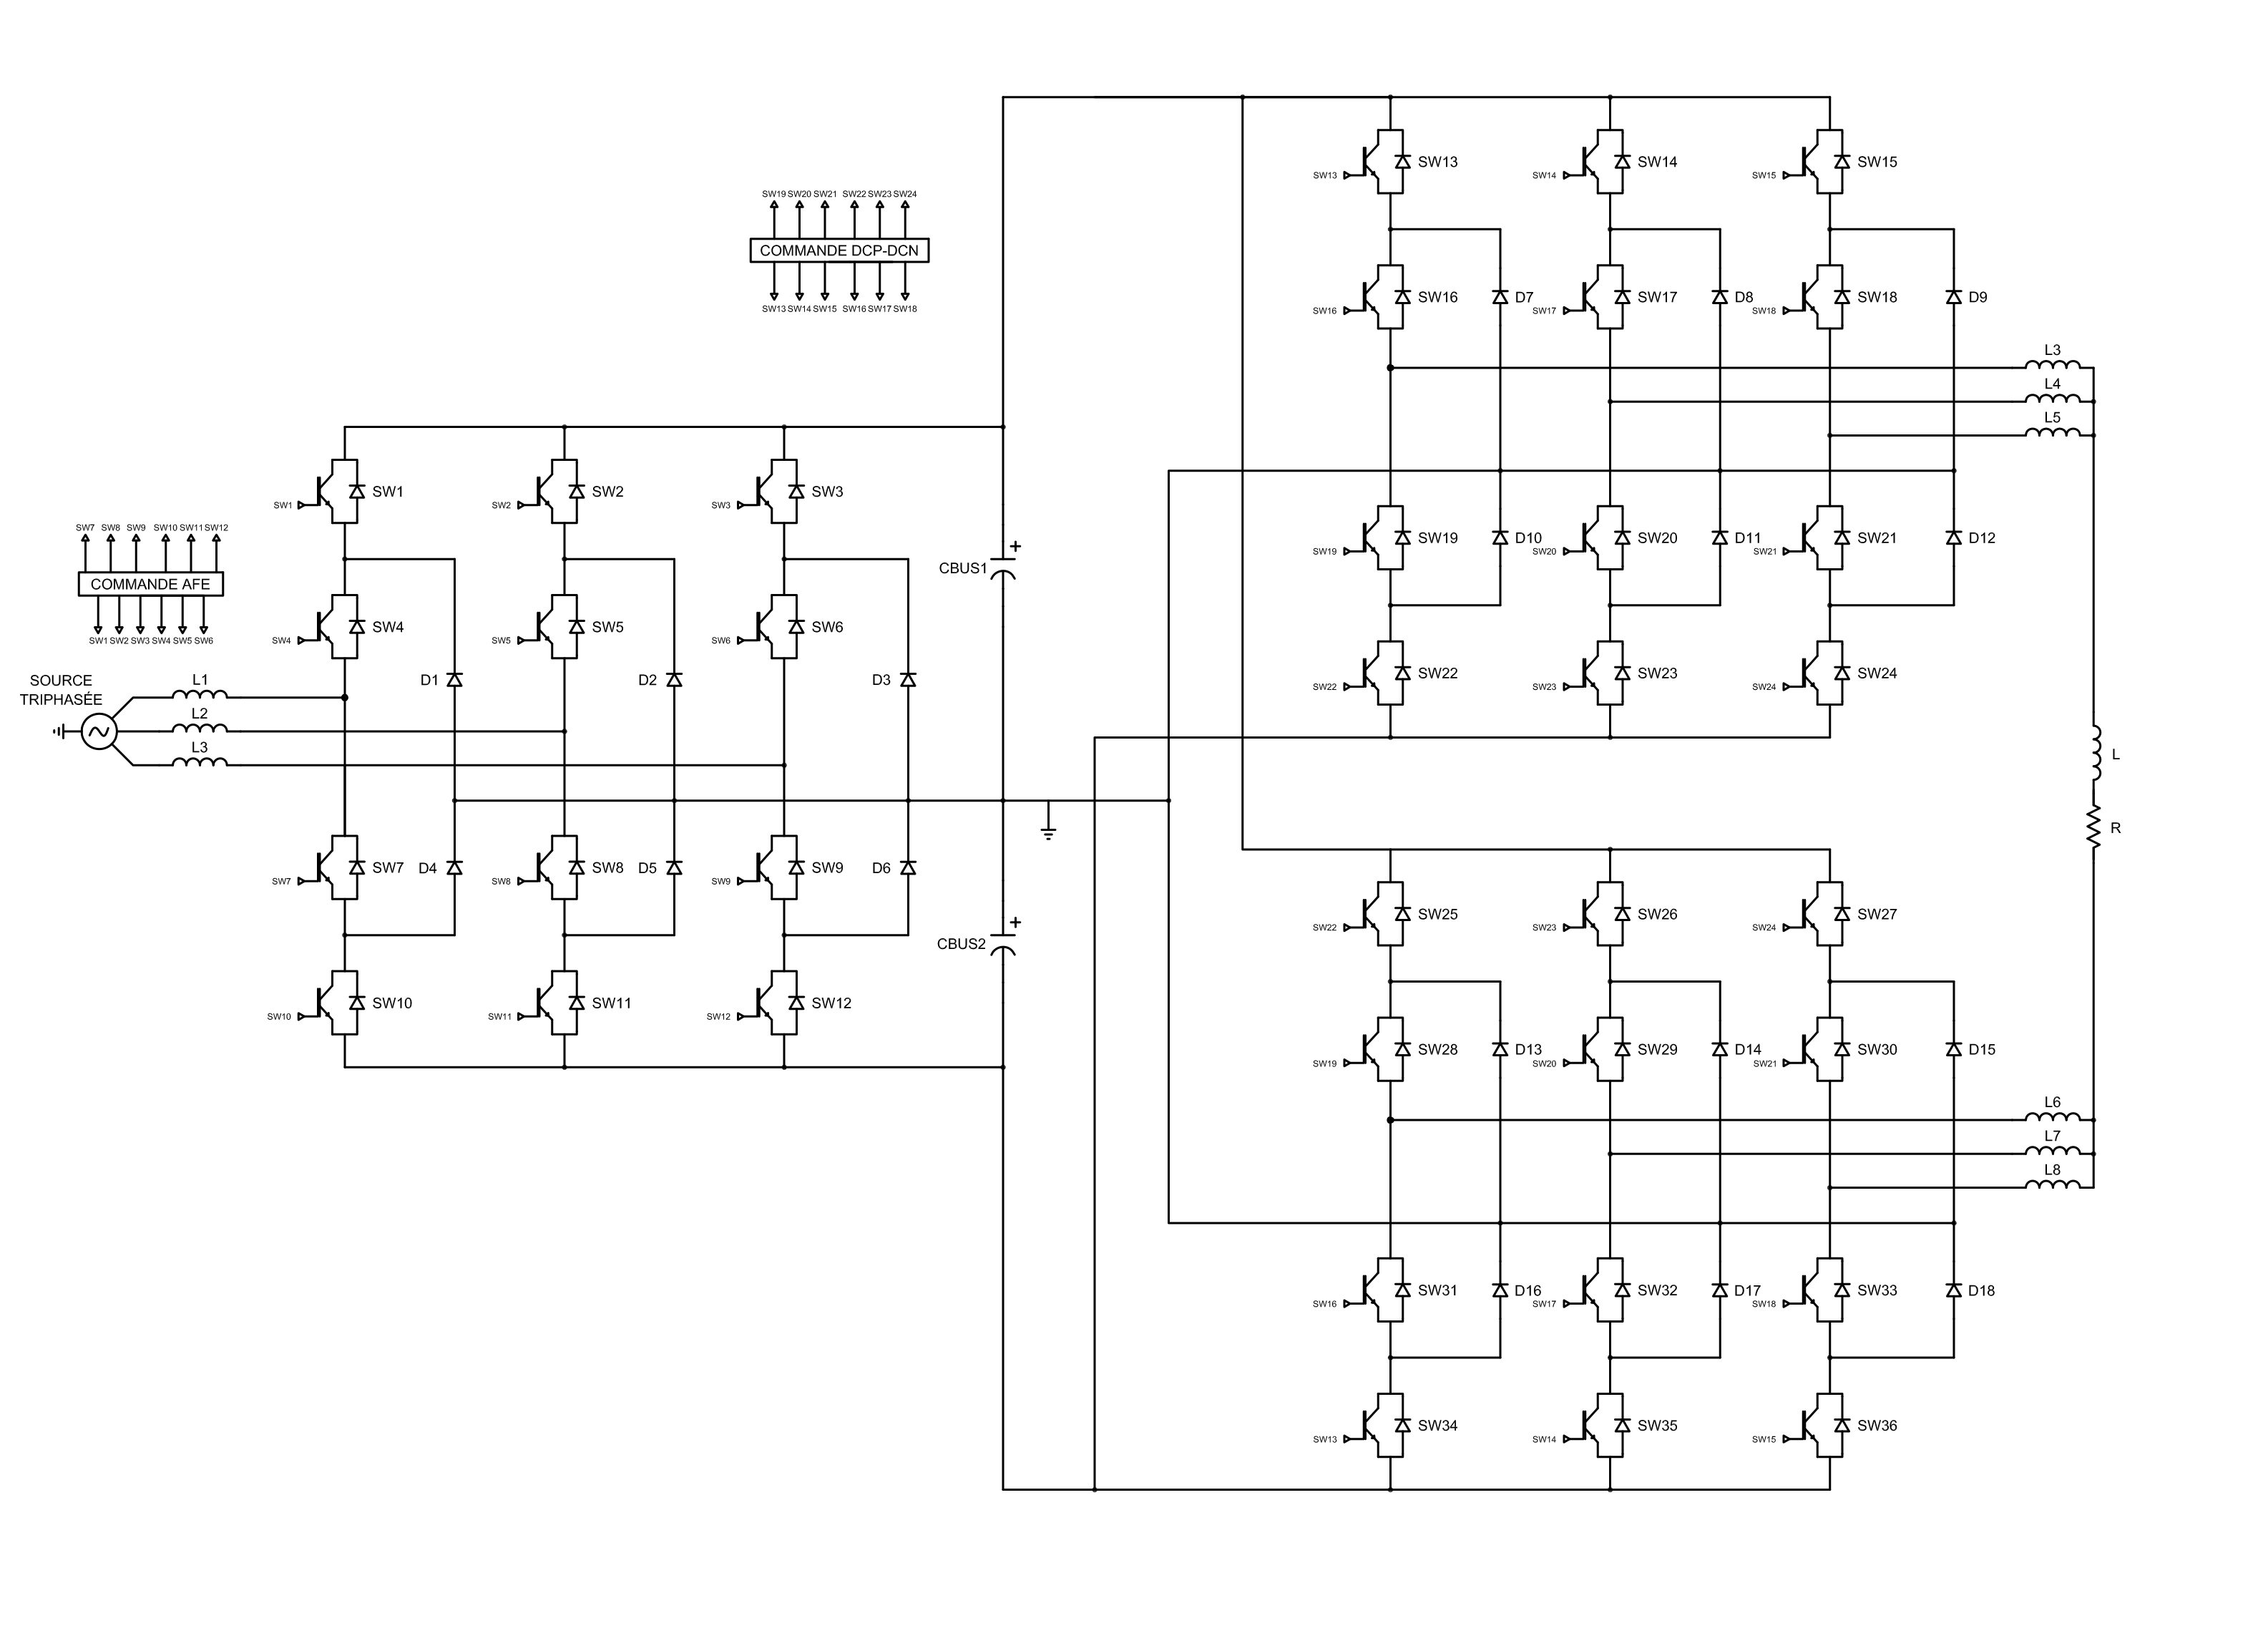
\includegraphics[scale=0.6]{fig/AFE_3L_RC_DCP_DCN.png}}
\caption{Circuit électrique de l'AFE 3 niveaux avec contrôle par hystérésis avec le DCP/DCN}
\label{circuit_AFE_3L_RC_DCP_DCN}
\end{figure}


\begin{table}[htb]
\centering
\begin{tabular}{|l|c|} 
  \hline
  \textbf{Paramètre} & \textbf{Valeur}  \\
  \hline\hline \hline
  \multicolumn{2}{|l|}{\textbf{AFE 3 niveaux}}\\ \hline \hline 
  Tension référence CC & 5000 V\\ \hline
  Fréquence de modulation & 1000 Hz \\ \hline
  Inductance côté AC& 814.87 $\mu$H\\ \hline
  Courant maximal à l'entrée& 800A \\ \hline \hline
  \multicolumn{2}{|l|}{\textbf{IGBT AFE}}\\ \hline
  Résistance interne & 0.001 $\Omega$\\
  Résistance du snubber & 100k $\Omega$\\ \hline \hline
   \multicolumn{2}{|l|}{\textbf{PI tension AFE}}\\ \hline
  Gain proportionnel & 282.9218 \\
  Gain intégrateur & 92.59 \\ \hline \hline
  \multicolumn{2}{|l|}{\textbf{PI courant AFE}}\\ \hline
  Gain proportionnel & 2 \\
  Gain intégrateur & 8 \\ \hline \hline
  \multicolumn{2}{|l|}{\textbf{PI commande AFE}}\\ \hline
  Rapport cyclique maximal & 0.95\\
  Gain proportionnel & 7.5e-4 \\
  Gain intégrateur & 0.005 \\ \hline \hline
  \multicolumn{2}{|l|}{\textbf{Bus CC}}\\ \hline
  Capacité & 330 mF\\
  \hline \hline \hline
  
  \multicolumn{2}{|l|}{\textbf{DCP/DCN}}\\ \hline \hline
  Fréquence de modulation & 333 Hz\\ \hline
  Rapport cyclique maximal & 1 \\ \hline
  Inductance de couplage & 10e-6 H \\ \hline \hline
  \multicolumn{2}{|l|}{\textbf{IGBT DCP/DCN}}\\ \hline
  Résistance interne & 0.001 $\Omega$\\
  Résistance du snubber & 100k $\Omega$\\ \hline \hline
   \multicolumn{2}{|l|}{\textbf{PI DCP/DCN}}\\ \hline
  Gain proportionnel & 1.5611 \\
  Gain intégrateur & 24.6 \\ \hline \hline
  \multicolumn{2}{|l|}{\textbf{Charge}}\\ \hline
  Résistance & 0.28 $\Omega$\\
  Inductance & 0.1 H \\
  \hline
\end{tabular}
\caption{Paramètres de simulation pour le DCP/DCN avec l'AFE 3 niveaux}
\label{p_AF_DCP}
\end{table}
\clearpage

\subsection{Résultats de simulation pour SPS et PSIM pour un pas de calcul de 1$\mu$s}
Cette section présente les résultats de simulations pour le système complet formé de l'AFE 3 niveaux avec régulation MLI et d'un convertisseur CC-CC composé de 2 cellules NPC 3 niveaux, pour un pas de calcul discret de 1$\mu$s. 

\begin{figure}[htb]
\makebox[\textwidth][c]{\includegraphics[scale=0.5]{fig/DCP_AFE/1u/cour_al.jpg}}
\caption{Le courant d'entrée de l'AFE pour un pas de calcul de 1$\mu$s}
\label{AF_DC_cou1}
\end{figure}


\begin{figure}[htb]
\makebox[\textwidth][c]{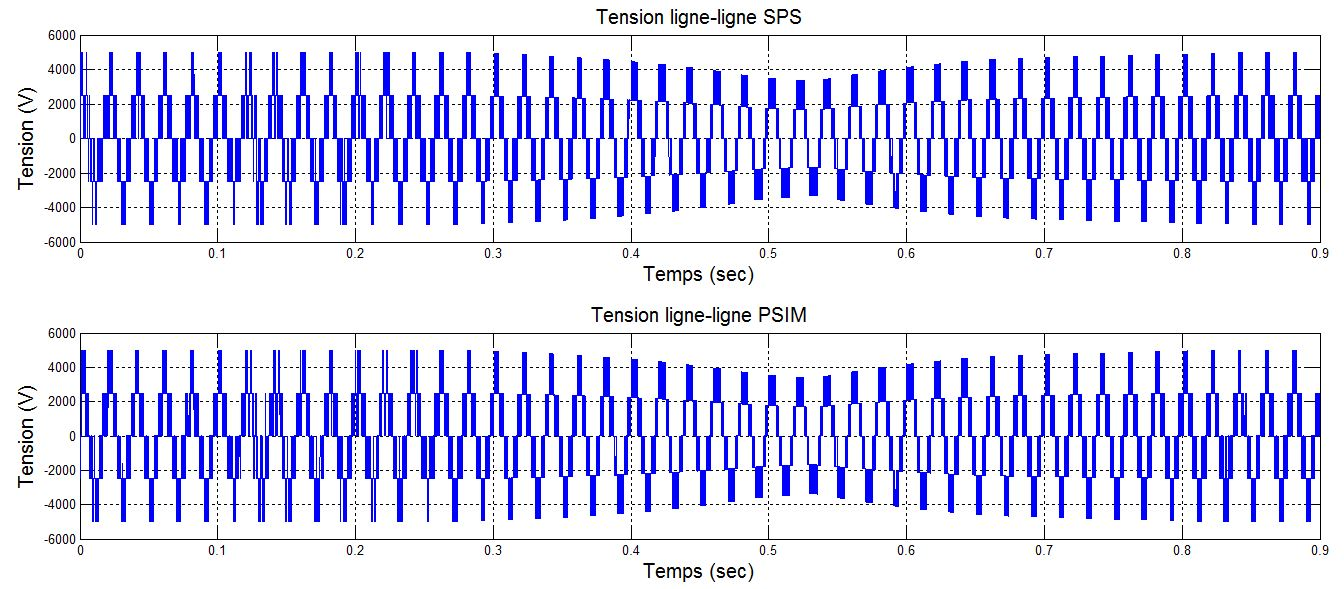
\includegraphics[scale=0.5]{fig/DCP_AFE/1u/ten_ligne_ligne.jpg}}
\caption{La tension ligne-ligne d'entrée de l'AFE pour un pas de calcul de 1$\mu$s}
\label{AF_DC_ten1}
\end{figure}


\begin{figure}[htb]
\makebox[\textwidth][c]{\includegraphics[scale=0.5]{fig/DCP_AFE/1u/ten_bus.jpg}}
\caption{La tension du bus CC pour un pas de calcul de 1$\mu$s}
\label{AF_DC_vch1}
\end{figure}



\begin{figure}[htb]
\makebox[\textwidth][c]{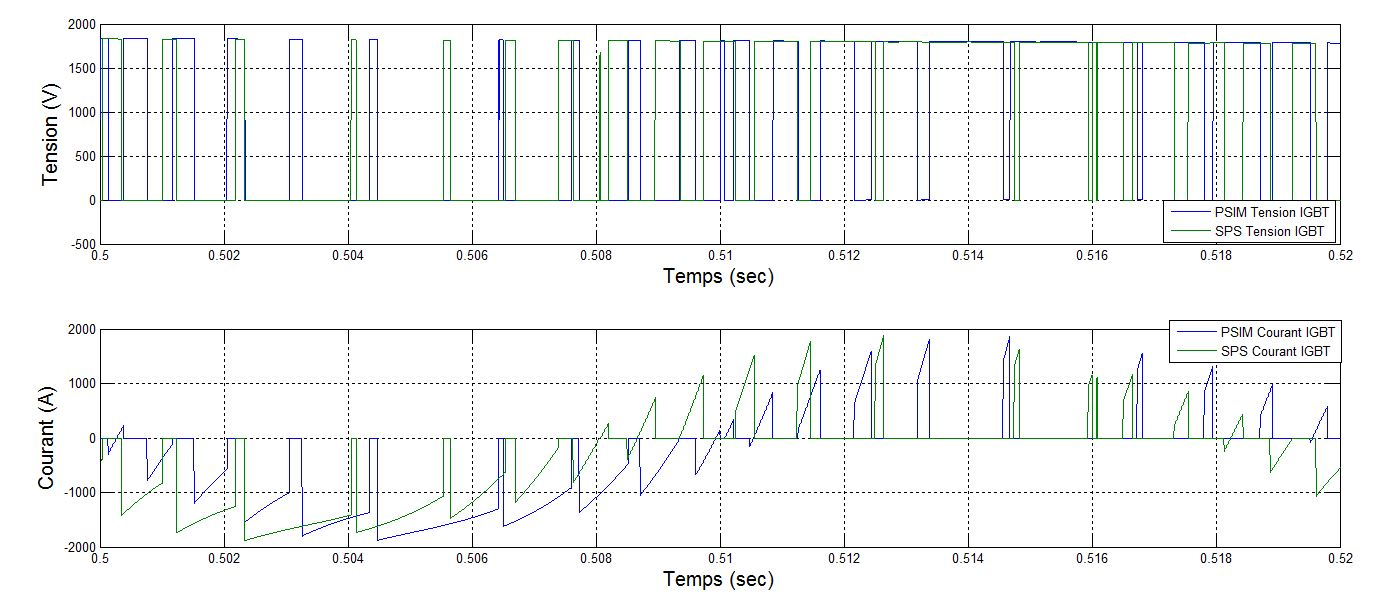
\includegraphics[scale=0.5]{fig/DCP_AFE/1u/IGBT_afe.jpg}}
\caption{La tension aux bornes d'un IGBT de l'AFE pour un pas de calcul de 1$\mu$s}
\label{AF_DC_IGBT1}
\end{figure}


\begin{figure}[htb]
\makebox[\textwidth][c]{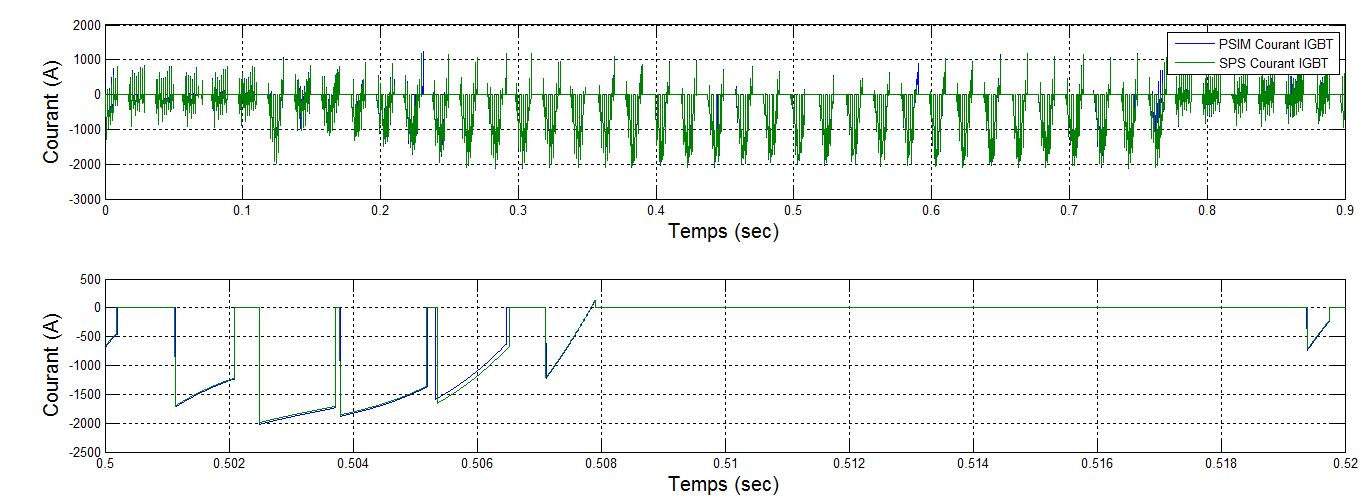
\includegraphics[scale=0.5]{fig/DCP_AFE/1u/cou_IGBT_afe.jpg}}
\caption{Le courant aux bornes d'un IGBT de l'AFE pour un pas de calcul de 1$\mu$s}
\label{AF_DC_IGBT2}
\end{figure}


\begin{figure}[htb]
\makebox[\textwidth][c]{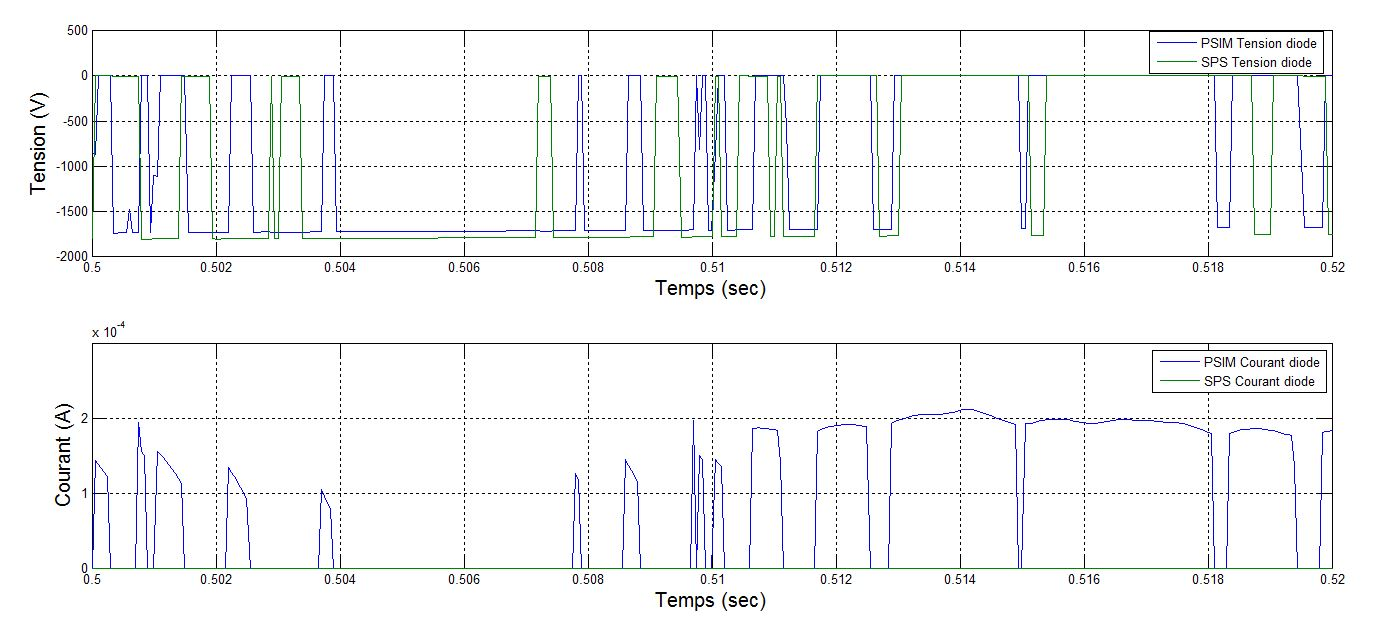
\includegraphics[scale=0.5]{fig/DCP_AFE/1u/ten_diode_afe.jpg}}
\caption{La tension aux bornes d'une diode de point milieu de l'AFE à 1$\mu$s}
\label{AF_DC_DI1}
\end{figure}


\begin{figure}[htb]
\makebox[\textwidth][c]{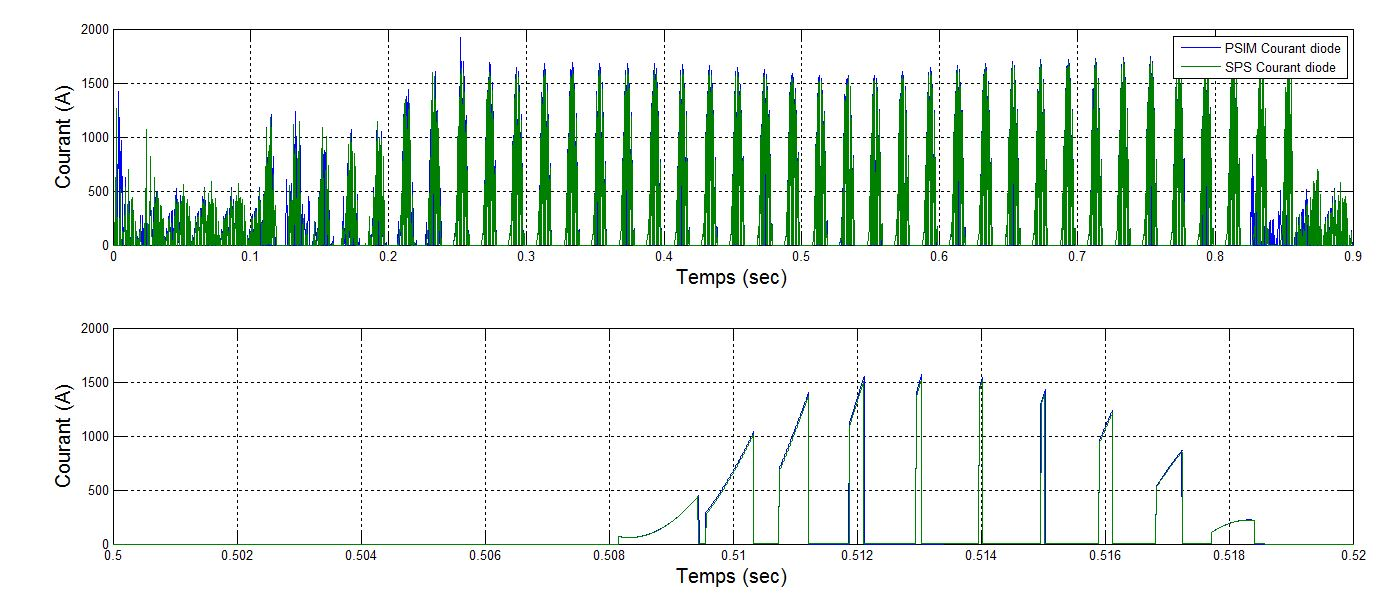
\includegraphics[scale=0.5]{fig/DCP_AFE/1u/cou_diode_afe.jpg}}
\caption{Le courant aux bornes d'une diode de point milieu de l'AFE à 1$\mu$s}
\label{AF_DC_DI2}
\end{figure}


\begin{figure}[htb]
\makebox[\textwidth][c]{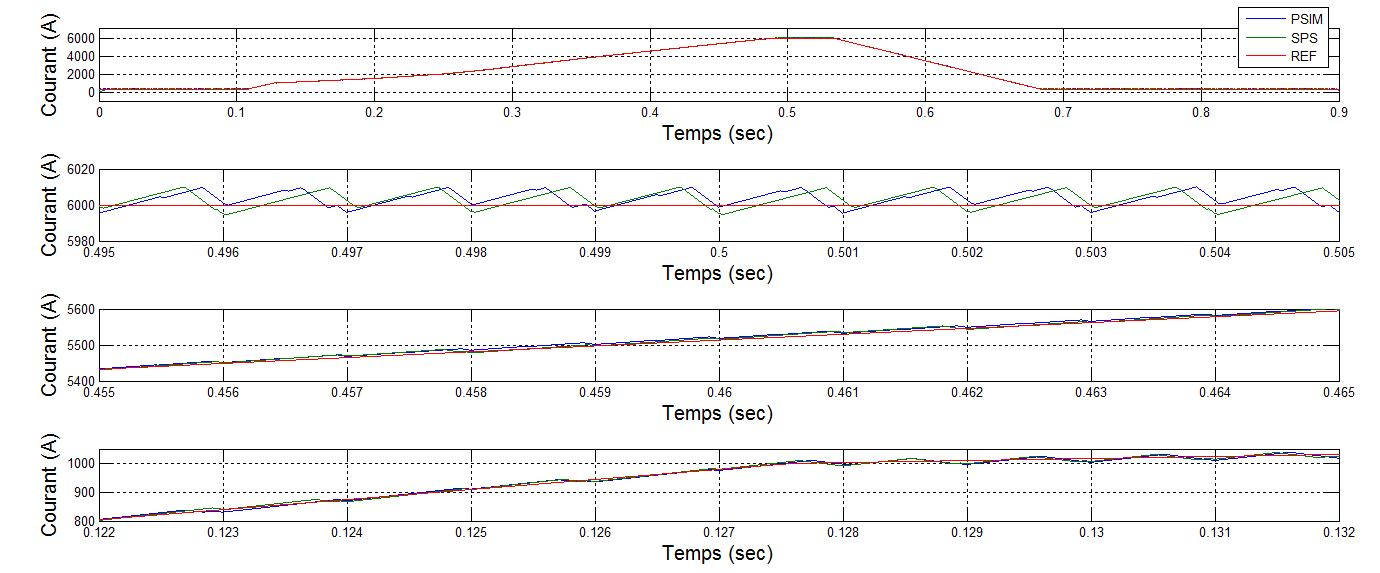
\includegraphics[scale=0.5]{fig/DCP_AFE/1u/cour_ch.jpg}}
\caption{Le courant aux bornes des électroaimants pour un pas de calcul de 1$\mu$s}
\label{AF_DC_CHA1}
\end{figure}



\begin{figure}[htb]
\makebox[\textwidth][c]{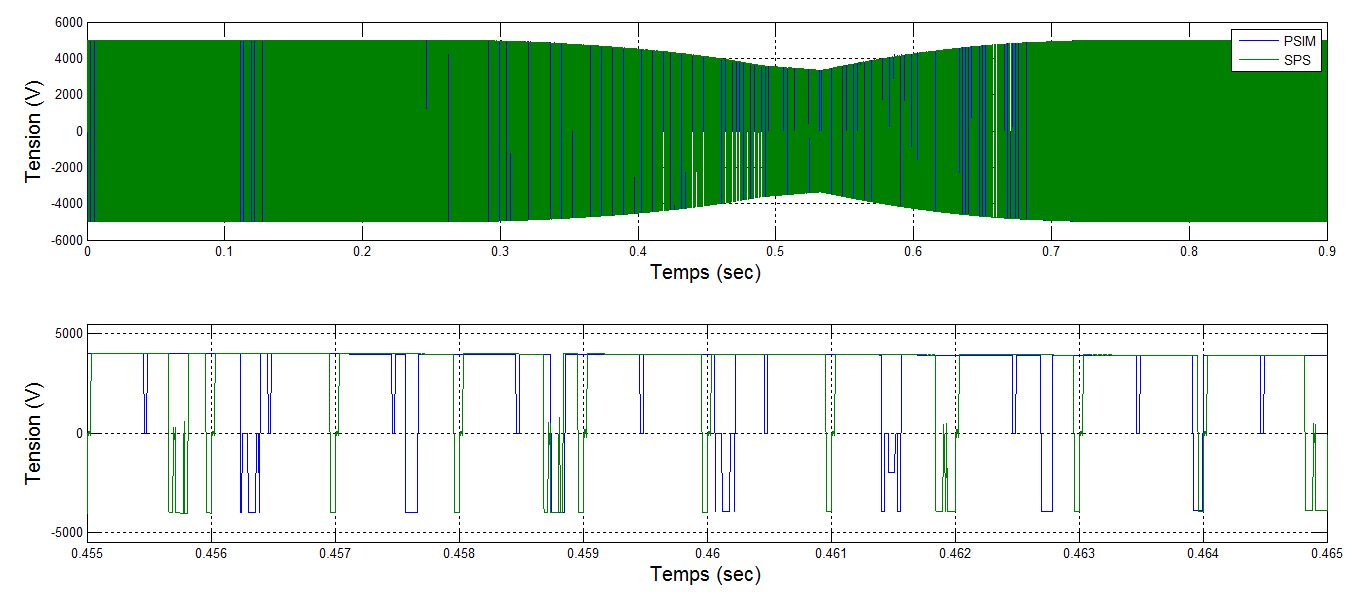
\includegraphics[scale=0.5]{fig/DCP_AFE/1u/ten_ch.jpg}}
\caption{La tension aux bornes des électroaimants pour un pas de calcul de 1$\mu$s}
\label{AF_DC_CHV1}
\end{figure}



\begin{figure}[htb]
\makebox[\textwidth][c]{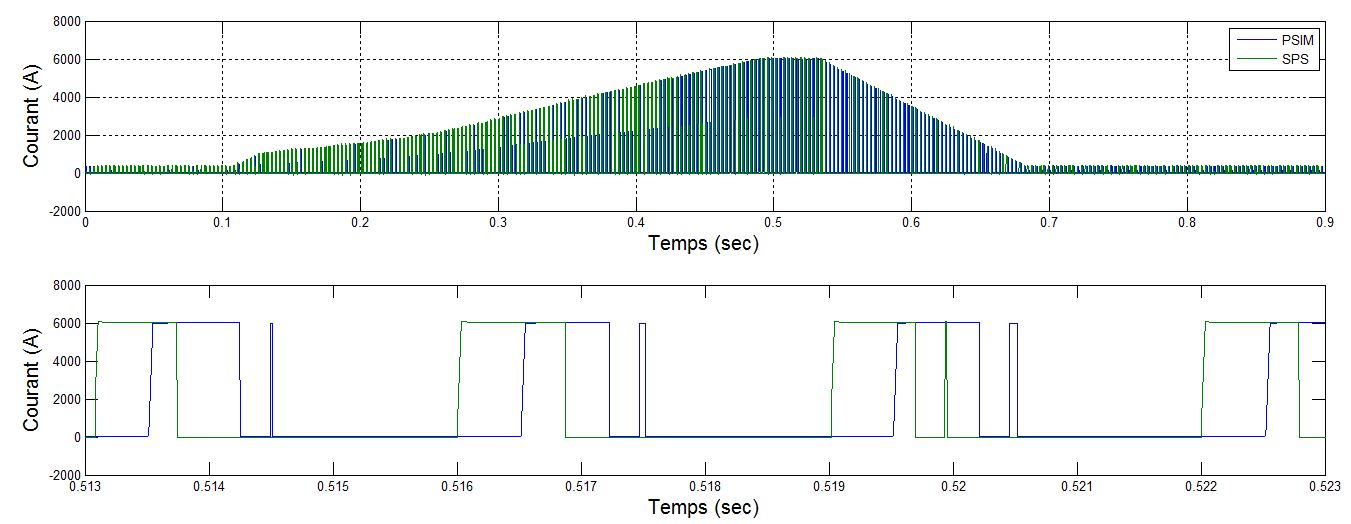
\includegraphics[scale=0.5]{fig/DCP_AFE/1u/hash_cou_IGBT.jpg}}
\caption{Le courant traversant un IGBT du DCP/DCN pour un pas de calcul de à 1$\mu$s}
\label{AF_DC_HAA1}
\end{figure}



\begin{figure}[htb]
\makebox[\textwidth][c]{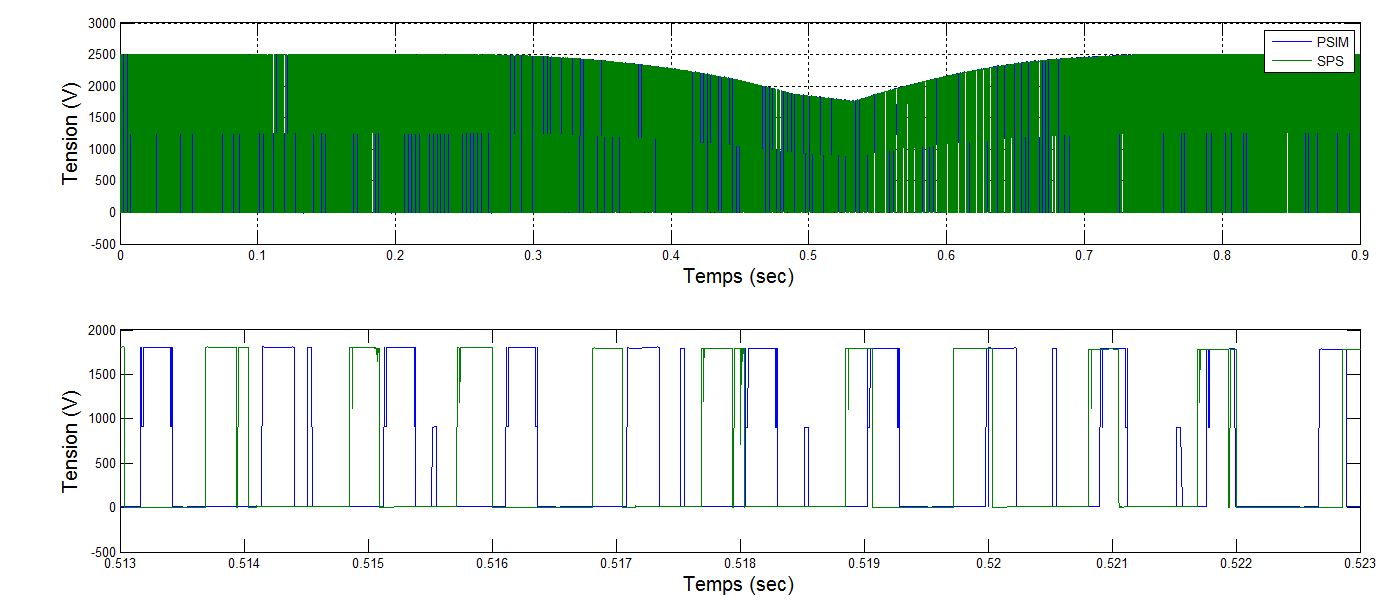
\includegraphics[scale=0.5]{fig/DCP_AFE/1u/hash_ten_IGBT.jpg}}
\caption{La tension aux bornes d'un IGBT du DCP/DCN pour un pas de calcul de 1$\mu$s}
\label{AF_DC_HAV1}
\end{figure}



\begin{figure}[htb]
\makebox[\textwidth][c]{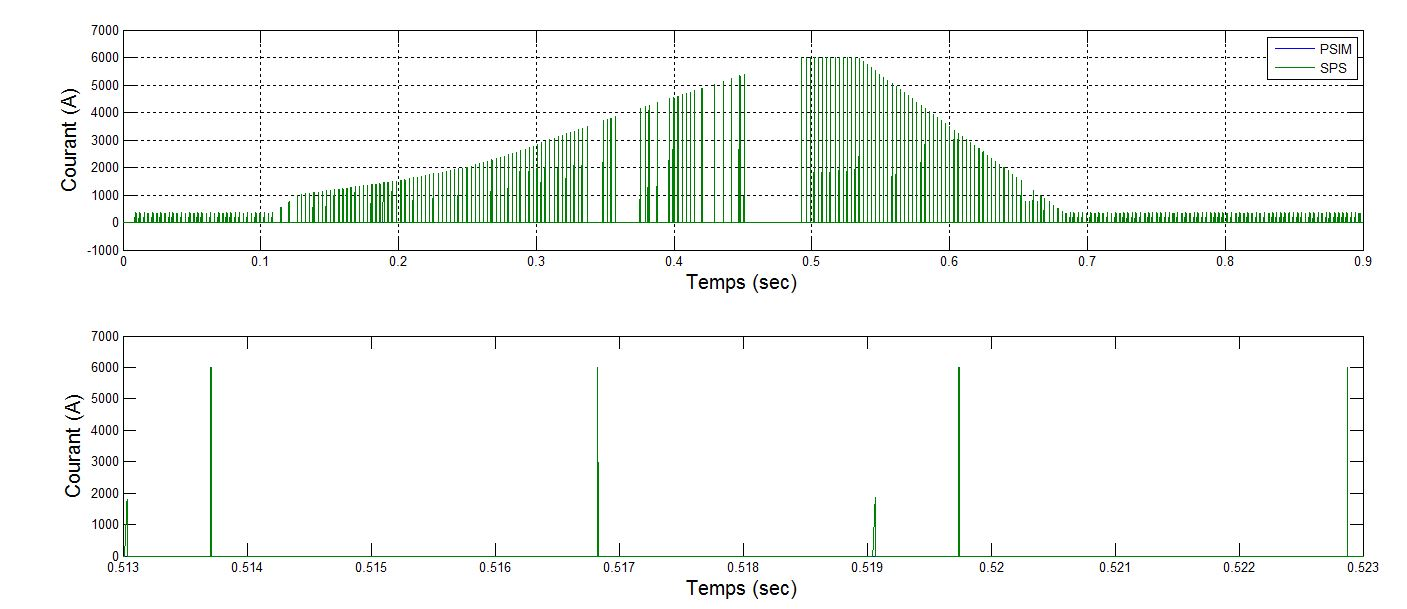
\includegraphics[scale=0.5]{fig/DCP_AFE/1u/hash_diode_cou.jpg}}
\caption{Le courant traversant une diode de point milieu du DCP/DCN pour un pas de calcul d 1$\mu$s}
\label{AF_DC_HA1}
\end{figure}


\begin{figure}[htb]

\makebox[\textwidth][c]{\includegraphics[scale=0.5]{fig/DCP_AFE/1u/hash_diode.jpg}}
\caption{La tension aux bornes d'une diode de point milieu du DCP/DCN pour un pas de calcul de 1$\mu$s}
\label{AF_DC_HV1}
\end{figure}
\clearpage


\subsection{Analyse des résultats comparatifs de SPS et de PSIM pour un pas de calcul de 1$\mu$s}
La figure \ref{AF_DC_cou1} présente le courant d'entrée de l'AFE débitant sur le bus CC avec le convertisseur CC-CC, formé de 2 cellules NPC 3 niveaux. On remarque que les formes de courant sont similaires, 	que les amplitudes pratiquement identiques et que le déphasage est minime. On en conclut donc que la méthode de modulation par MLI offre des performances, à toutes fins pratiques, identiques dans les 2 simulateurs.
La tension du bus CC est présentée à la figure \ref{AF_DC_vch1}. Sur cette figure, on remarque bien que la tension du bus CC chute pendant l'appel de puissance côté charge. On note que les 2 simulateurs réagissent de manière similaire, malgré les 36 IGBT et les 18 diodes en jeu. On comprend donc que l'implantation des modèles dans les 2 simulateurs permet d'obtenir des résultats similaires. L'erreur à constater est de l'ordre de 200V, tout comme l'implantation précédente. Vu le nombre de composantes et les différences d'implantations, il est plutôt difficile de pointer une cause exacte. Les sous-modèles étant eux-même différents, on ne constate pas d'augmentation significative de l'erreur, ce qui permet de conclure sur la véracité des résultats. 
La figure \ref{AF_DC_ten1} présente la tension ligne-ligne vue à l'entrée de l'AFE. On constate ici la souplesse apportée par un redresseur 3 niveaux, soit un niveau intermédiaire de 2.5kV qui permet de minimiser la tension instantanée pour représenter l'onde de tension. On comprend qu'il devient alors intéressant de disposer de plusieurs niveaux afin d'être le plus près possible de la tension désirée, tout en minimisant les tensions vues aux interrupteurs.
Les figures \ref{AF_DC_IGBT1} et \ref{AF_DC_IGBT2} présentent respectivement le courant et la tension d'un des IGBT de l'AFE. On constate que les patrons de courant sont similaires, tout comme les moments d'amorçages. Le décalage est difficile à remarquer à l'oeil et on peut juger que les différences sont mineures entre les 2 simulations. 
Les figures \ref{AF_DC_DI1} et \ref{AF_DC_DI2} présentent respectivement le courant et la tension d'une diode de point milieu de l'AFE. Tout comme dans le cas précédent, on remarque que les patrons sont similaires, mais avec ces résultats, on constate un décalage entre les formes de courants et des points de tension différents. Les erreurs sont difficilement perceptibles à l'oeil. 
La figure \ref{AF_DC_CHA1} présente le courant dans la charge pendant un cycle d'impulsion, celui en montée initiale, en montée rapide et en maintien. Tout comme dans le cas du DCP/DCN, on remarque que la fréquence des oscillations de courant vues à la charge change selon les simulateurs et que les 2 signaux glissent l'un par rapport à l'autre. Les oscillations sont de même amplitude, mais elles se décalent l'une par rapport à l'autre.
Les observations pour les interrupteurs du convertisseur CC-CC sont les mêmes que celles énoncées pour l'AFE. On remarque des patrons similaires, mais des décalages en temps.
\clearpage

\section{Analyse du fonctionnement du système intégré}
Cette section correspond au point culminant du projet. La méthodologie ayant été respectée dans les précédents modèles, la construction du simulateur complet est fondée sur la compréhension acquise dans les constructions élémentaires. Ce modèle est une approximation permettant d'observer la dynamique du système comprenant des convertisseurs 3 niveaux. L'objectif ici n'est pas de documenter les sources d'erreurs, mais d'observer la dynamique globale et de comprendre les motifs liés aux contraintes physiques des systèmes implantés. La puissance traitée étant relativement élevée, les interrupteurs sont à la fois amenés à des contraintes de puissance élevées, mais aussi à des contraintes de longévité et de fiabilité. L'utilisation du modèle complet, qui est une évolution des sous-modèles présentés précédemment, permet avant tout de mettre en perspective l'impact de la charge sur le réseau qui est minimisé par l'usage d'un banc de capacité d'envergure. La pulsation de 18MW crête est fournie en grande partie par le banc de condensateur. L'AFE 3 niveaux permet à tout le moins de ramener la tension du bus à 5kV, suivant une baisse de tension causée par la demande croissante de puissance pendant la pulsation. Un AFE plus lent provoque une baisse plus marquée de la tension du bus CC, mais une perturbation moins marquée du côté du réseau. Cependant, l'atteinte du régime permanent, en ce qui a trait à la tension du bus CC est plus longue et limite la fréquence des cycles. Par ailleurs, d'un point de vue économique, il est relativement plus simple d'augmenter la taille du banc de condensateurs (formés d'éléments simples) que d'utiliser des interrupteurs avec une température de jonction plus élevée. La fiabilité des interrupteurs est aussi en cause, puisqu'une augmentation de la température de jonction (causée par un appel de puissance instantanée plus grand) est néfaste pour leur durée de vie. L'objectif du système intégré est donc d'offrir un compromis entre la durée de vie des interrupteurs, le nombre de cycles répétitifs et les perturbations vues du réseau. Il est intéressant d'ajouter que l'entrelacement de la commande des interrupteurs minimise le temps de conduction de ceux-ci et favorise la durée de vie, tout en minimisant l'échauffement nominal. L'objectif des ingénieurs du CERN étant de maintenir la température des composantes dans une plage limitée. L'usage de 2 cellules permet  la réversibilité en courant en plus d'une augmentation de la tension applicable à la charge. En effet, afin de pouvoir  maintenir une rampe de courant constante à la charge, il est nécessaire qu'au point le plus bas de la tension, le plus élevé pour le courant, la tension moyenne accessible par le convertisseur soit suffisante. La tension du bus CC suivant une baisse comprise entre 1.8kV et 2kV, le pont DCP/DCP doit tout juste atteindre sa limitation de rapport cyclique à ce point. Autrement dit, on comprend que le bus CC est choisi selon 2 critères: vitesse de décharge (capacité en F) et tension nominale, selon la chute de tension et la tension moyenne maximale. Utiliser une tension du bus CC plus grande implique une réduction de la marge de sécurité pour les interrupteurs qui sont déjà dans les plus performants sur le marché. On constate donc que, suivant le point nominal souhaité des interrupteurs, on dimensionne la tension du bus CC et par la suite, la capacité nécessaire afin de maintenir une tension suffisante pour la charge. Comme les bancs de condensateurs sont des technologies éprouvées et plus abordables que des cellules NPC 3 niveaux, il est plus intéressant de choisir un banc de condensateur avec une plus grande capacité que d'associer davantage d'interrupteurs.
